\documentclass[10pt,twocolumn,letterpaper]{article}

\usepackage{cvpr}              % To produce the CAMERA-READY version

% Include other packages here, before hyperref.
\usepackage{graphicx}
\usepackage{amsmath}
\usepackage{amssymb}
\usepackage{booktabs}
\usepackage{rotating}
\usepackage{makecell}
%\usepackage{endfloat}  # adding this won't show figures


% It is strongly recommended to use hyperref, especially for the review version.
% hyperref with option pagebackref eases the reviewers' job.
% Please disable hyperref *only* if you encounter grave issues, e.g. with the
% file validation for the camera-ready version.
%
% If you comment hyperref and then uncomment it, you should delete
% ReviewTempalte.aux before re-running LaTeX.
% (Or just hit 'q' on the first LaTeX run, let it finish, and you
%  should be clear).
\usepackage[pagebackref,breaklinks,colorlinks]{hyperref}


% Support for easy cross-referencing
\usepackage[capitalize]{cleveref}
\crefname{section}{Sec.}{Secs.}
\Crefname{section}{Section}{Sections}
\Crefname{table}{Table}{Tables}
\crefname{table}{Tab.}{Tabs.}


%%%%%%%%% PAPER ID  - PLEASE UPDATE
\def\cvprPaperID{*****} % *** Enter the CVPR Paper ID here
\def\confName{CVPR}
\def\confYear{2022}


\begin{document}

%%%%%%%%% TITLE - PLEASE UPDATE

%% TODO(adrs): Update Title to represent the hypothesis we actually tested
\title{Comparing Transformers and CNNs on the SpaceNet Flood Detection Challenge}

\author{Adrian Stoll\\
Stanford University\\
{\tt\small adrs@stanford.edu}
\and
Naijing Guo\\
Stanford University\\
{\tt\small njguo@stanford.edu}
\and
Nenad Bozinovic\\
Stanford University\\
{\tt\small nesa@stanford.edu}
}
\maketitle

%%%%%%%%% ABSTRACT
\begin{abstract}

This project explores the SpaceNet8 Challenge, which aims to detect floods caused by hurricanes and heavy rains. We compared a variety of transformer and CNN segmentation architectures. We found that large pre-trained Segformer models had better performance than Resnet and U-net based models despite consuming more computational resources. The highest IoU for building detection was 61\% for Segformer, which indicated that attention is better suited for detecting building-footprints than convolutions. We noticed that flooded road detection was particularly hard with highest IoU of 40\%. We observed pre-training on ImageNet and Cityscapes datasets provided a moderate improvement compared to pre-training on the ADE20k dataset and a significant improvement compared to training a model from scratch.

\end{abstract}

%%%%%%%%% BODY TEXT
\section{Introduction}
\label{sec:intro}

Floods are among the most devastating natural disasters, causing significant damage to buildings, infrastructure, and human life, as well as exacerbating environmental problems such as erosion and land degradation. Remote sensing, specifically satellite imagery analysis, has become a vital tool for flood detection and monitoring, providing fast initial mapping of flooded regions and helping in post-disaster assessments. 

The SpaceNet8 Challenge \cite{spacenet8} aims at developing open-source computer vision and machine learning methods for remote sensing data in the context of floods caused by hurricanes and heavy rains. The goal of this challenge is to rapidly develop maps and analyze the scale of destruction to better direct resources and first responders in real-world disaster scenarios by leveraging the existing repository of datasets and algorithms from SpaceNet Challenges 1-7 and expanding to multiclass feature extraction and characterization. We use the SpaceNet 8 dataset which has two sets of images, namely pre-event images and post-event images. We have two independently trained models. The first model is the foundational features network which takes the pre-event images as inputs and segments buildings and roads. This network returns two outputs with the same size as the original image and different number of channels - road speed that has 8 channels and building that has 1 channel. The second model is the flood network that takes both pre and post-event images as input and outputs predictions of flood status. The outputs have the same spatial dimensions as the the input image with 4 channels: flooded building, non-flooded building, flooded road, and non-flooded road. We investigated a few model options including transformer based and U-Net based models. 




% Explain the problem and why it is important. Discuss your motivation for pursuing this problem. Give some background if necessary. Clearly state what the input and output is. Be very explicit: “The input to our algorithm is a {image, video, patient age, 3D video, etc.}. We then use a {SVM, CNN, GAN, etc.} to output a predicted {age, cancer type, restaurant, ramen, etc.}.” This is very important since different teams have different inputs/outputs spanning different application domains. Being explicit about this makes it easier for readers.

\section{Related Work}
\label{sec:related}

Works related to automated detection and identification of buildings in off-nadir satellite imagery can be generally divided into three categories - deep learning based approach, Object-Based Image Analysis (OBIA), and hybrid approaches. In this section, we discuss their strengths and weaknesses.

\subsection{Deep Learning Based Approach}

\subsubsection{Deeplab Approach}

The Deeplab model \cite{deeplab7913730} uses a few novel approaches to address the issues in semantic image segmentation. It takes advantage of upsampled filters - also known as 'atrous convolution' - to better control the resolution and incorporate larger context without increasing the number of parameters or the amount of computation. It also uses fully connected Conditional Random Field (CRF) to improve localization performance. And overall this approach has improved performance in delineating object boundaries, but has rough final segmentation results due to the lacks of considering low-level feature images with rich detailed information \cite{wang2022improved}. 

\subsubsection{U-Net Based Approaches} 

 U-Net is an encoder-decoder convolutional neural network that is a widely-used for semantic segmentation \cite{ronneberger2015unet}. The network was first developed for application in biomedical image segmentation and was later extended to various fields including remote sensing analyses. Its inherent strengths lie in its ability to effectively learn and capture local information through the combination of encoder and decoder architectures. However, in general U-Net struggles to grasp global contextual information, which can limit its performance \cite{shahedi2020study}.

\subsection{Object-Based Image Analysis}

Object-Based Image Analysis, like U-Net, was also originated from applications in biological image scans and later evolved into Geographic Object-Based Image Analysis that is used on remote sensing \cite{blaschke2010object}. OBIA involves segmenting images into meaningful homogeneous regions or objects, which are further analyzed by feature and context extraction. This approach can better handle multiscale and heterogeneity problems, but requires extensive domain knowledge and a finely-tuned thresholding mechanism \cite{Hay2006ObjectbasedIA}.

\subsection{Hybrid Approaches}


 A hybrid approach combining CNNs and OBIA was proposed in the research area of ecology to better monitor the changes in vegetation cover on very high-resolution images \cite{guirado2021mask}. The CNN extracts feature maps, which are fed into an OBIA module to refine the segmentation results. This approach was proposed to resolve the issue that the model performance could be affected by the spatial resolution of the orthoimages utilized, which presents in both CNN and OBIA based models. However, this model requires numerous high-quality high-resolution images, which are not always accessible in various fields of applications. 

\subsection{State-of-the-Art: SAM}

The Segment Anything Model (SAM) is a groundbreaking image segmentation model that is is built upon a MAE pre-trained Vision Transformer model. It is designed to segment objects in images using zero-shot learning, which means it can generalize across domains without additional training \cite{Kirillov2023SegmentA}. We will discuss the use of SAM in our project in a later section. 



% You should find existing papers, group them into categories based on their approaches, and talk about exemplary ones in each category: Discuss strengths and weaknesses. In your opinion, which approaches were clever/good? What is the state-of-the-art? Do most people perform the task by hand? You should aim to have at least 10 references in the related work. Include previous attempts by others at your problem, previous technical methods, or previous learning algorithms. Google Scholar is very useful for this: https://scholar.google.com/ (search your paper, and you can click “cite” to generate the BibTeX for it.) You can also try http://www.arxiv-sanity.com/ to search for recent arXiv papers.


\section{Dataset}
\label{sec:dataset}

We use SpaceNet8 dataset described in detail \href{https://openaccess.thecvf.com/content/CVPR2022W/EarthVision/papers/Hansch_SpaceNet_8_-_The_Detection_of_Flooded_Roads_and_Buildings_CVPRW_2022_paper.pdf}{here} \cite{spacenet8}. Data has been acquired using Maxar’s Earth observation satellites (data under creative common license). For SpaceNet8 dataset, two distinct areas of interest (AOIs) were selected that were flooded in 2021 (Germany and Louisiana). Data consists of pansharpened RGB (0.3-0.8m resolution) that are routinely published through Maxar Open Data Program.

Data was pre-labeled by analysts for both the pre- and post-event images. A road segment is considered flooded if it is visibly covered with water or rubble in the post-event imagery. If a building is assigned the flooded attribute, it means that there is flood water in its immediate proximity which is a proxy for probable flooding (since it is not possible from satellite imagery to determine whether a building is actually flooded inside). In the event that cloud cover obscured features in the post-event image, as is often the case in flooding disasters, analysts labeled only visible areas and not make any assumptions where features could not be seen (Figure \ref{fig:dataset}).

Pre- and post-event images do not overlap perfectly but are close enough for our purpose. Masks are build from GeoJSON data, where, for example, only vertices of the building polygon mask are stored, vs full mask image (more details \href{https://medium.com/the-downlinq/getting-started-with-spacenet-data-827fd2ec9f53}{here}).

\begin{figure}[t]
  \centering
   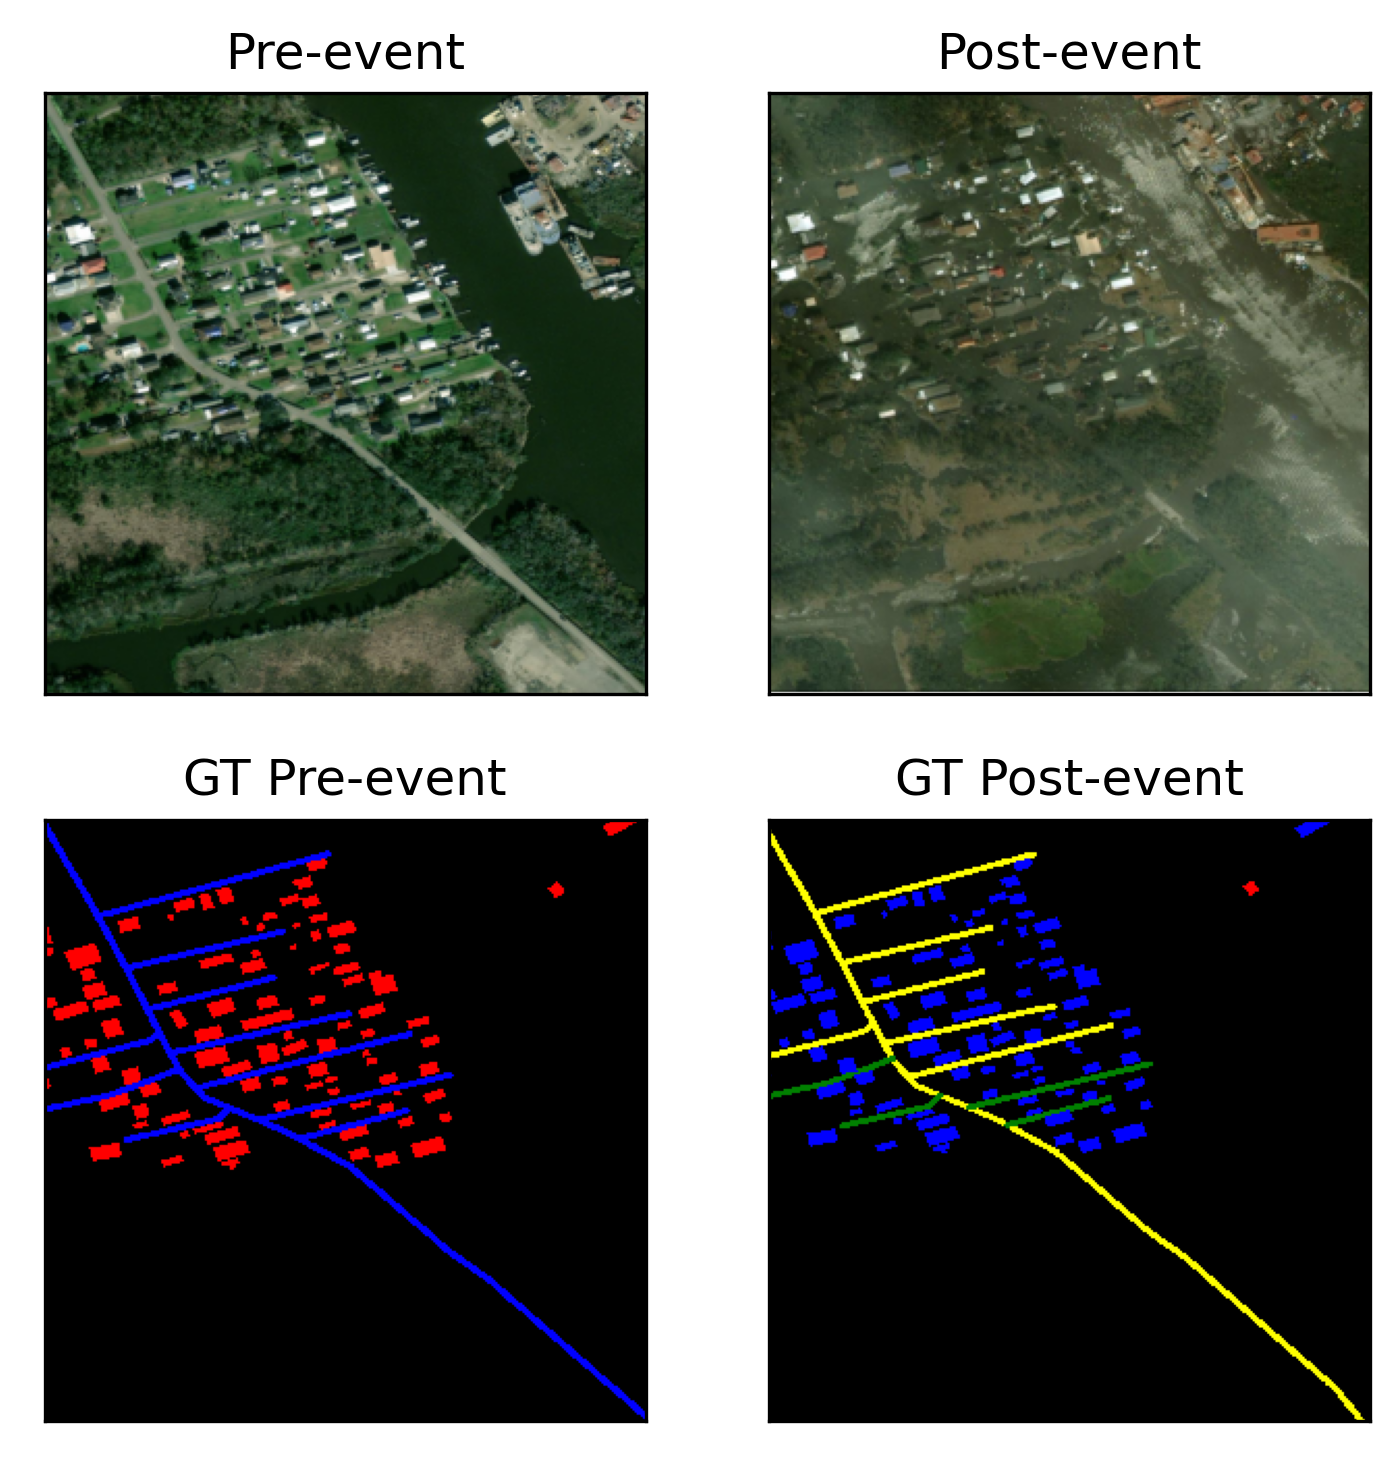
\includegraphics[width=1.0\linewidth]{figures/dataset.png}
   \caption{Examples of raw images pre- and post-event (top row) and respective ground truth segmenation masks (bottom row). Colors indicate classes (buildings, road, flooded buildings and flooded roads). In this example blue and yellow colors refer to flooded buildings and roads. For pre-event labels there is 1 building class and 8 road classes denoting speed (10 mph per class). For post event there are 4 classes (non-flooded building, flooded building, flooded road, non-flooded road).}
   \label{fig:dataset}
\end{figure}

At our disposal we had 801 labeled RGB images (1300x1300) and corresponding masks (Fig. \ref{fig:dataset}). The focus of this project was to try different models and we have opted against hyper-parameter optimization, hence we had no validation dataset, and kept 122 images (15\%) for testing. The images were not normalized or otherwise prepossessed before being fed into the models. All models were trained and evaluated using the same training-test split.


%Give details about your dataset: How many training/validation/test examples do you have? Is there any data preprocessing you did? What about normalization or data augmentation? What is the resolution of your images? You should also talk about the features you used. If you extracted features using Fourier transforms, word2vec, histogram of oriented gradients (HOG), PCA, ICA, etc. make sure to talk about it. Try to include examples of your data in the report (e.g. include an image, show a waveform, price graph, etc.).

\section{Pipeline}

We have developed a streamlined pipeline (training and evaluation) that enables easy experimentation. The result of each \textit{run} is a metrics file containing model name, parameter count, peak GPU memory usage, batch size, learning rate, per-epoch training and validation loss, as well as all Intersection-of-Union (IoU) metrics for each segmentation class and a best validation-loss model checkpoint.

Each model was trained on the entire training set for typically 10 epochs (45 min on A6000) after which we would typically see validation loss convergence and overfitting on the training dataset. Each training run used the Adam optimizer \cite{kingma2017adam} with a learning rate of 0.0001 and cross-entropy as the loss function. We used the maximum possible batch size that would fit in GPU memory.

For evaluation, each model ran inference on all of the validation images to produces segmentation masks yielding per-pixel-precision, recall, and F1 score, and ultimately Intersection-over-Union (IoU) percentage between prediction for each class (e.g. non-flooded building, flooded building) and its labeled masks. 

In the interest of time, we opted to modify the baseline pipeline provided by the Spacenet challenge organizers. The pipeline is notably different from most other pipelines as it uses two models: one for foundation feature detection (roads and buildings), and another so-called Siamese, encoder for flood detection. The architecture can be seen in Figure \ref{fig:baseline}. The foundation features network passes the images thought an encoder-decoder backbone followed by two sets of convolutions layers - one outputting building and the other road network predictions. The flood attribution network passes pre- and post-event images thought encoder-decoder backbones with shared weights (hence the name Siamese network) to extra image features. The flood network then concatenates these features together along the channel dimension and passes the features thought a sequence of convolution layers to output the flooded/not-flooded road/building predictions.

\section{Methods}
\label{sec:methods}

We experimented with various backbones for the flood network and Siamese foundation features network to compare the performance and characteristics of convolutional U-net and transformer model families. The families of models we evaluated include Segformer \cite{xie2021segformer}, DenseNet\cite{Huang2016DenselyCC}, and EfficientNet\cite{Tan_Le_2019}. The baseline the models were compared against is the reference SpaceNet pipeline \cite{spacenet8_baseline} with a Resnet34 backbone released by the competition organizers. We also experimented fine-tuning backbone models with pre-trained weights from ImageNet \cite{ILSVRC15}, ADE20k \cite{zhou2017scene}, and Cityscapes \cite{cordts2016cityscapes} datasets as well as training from scratch.

\begin{figure}[t]
  \centering
   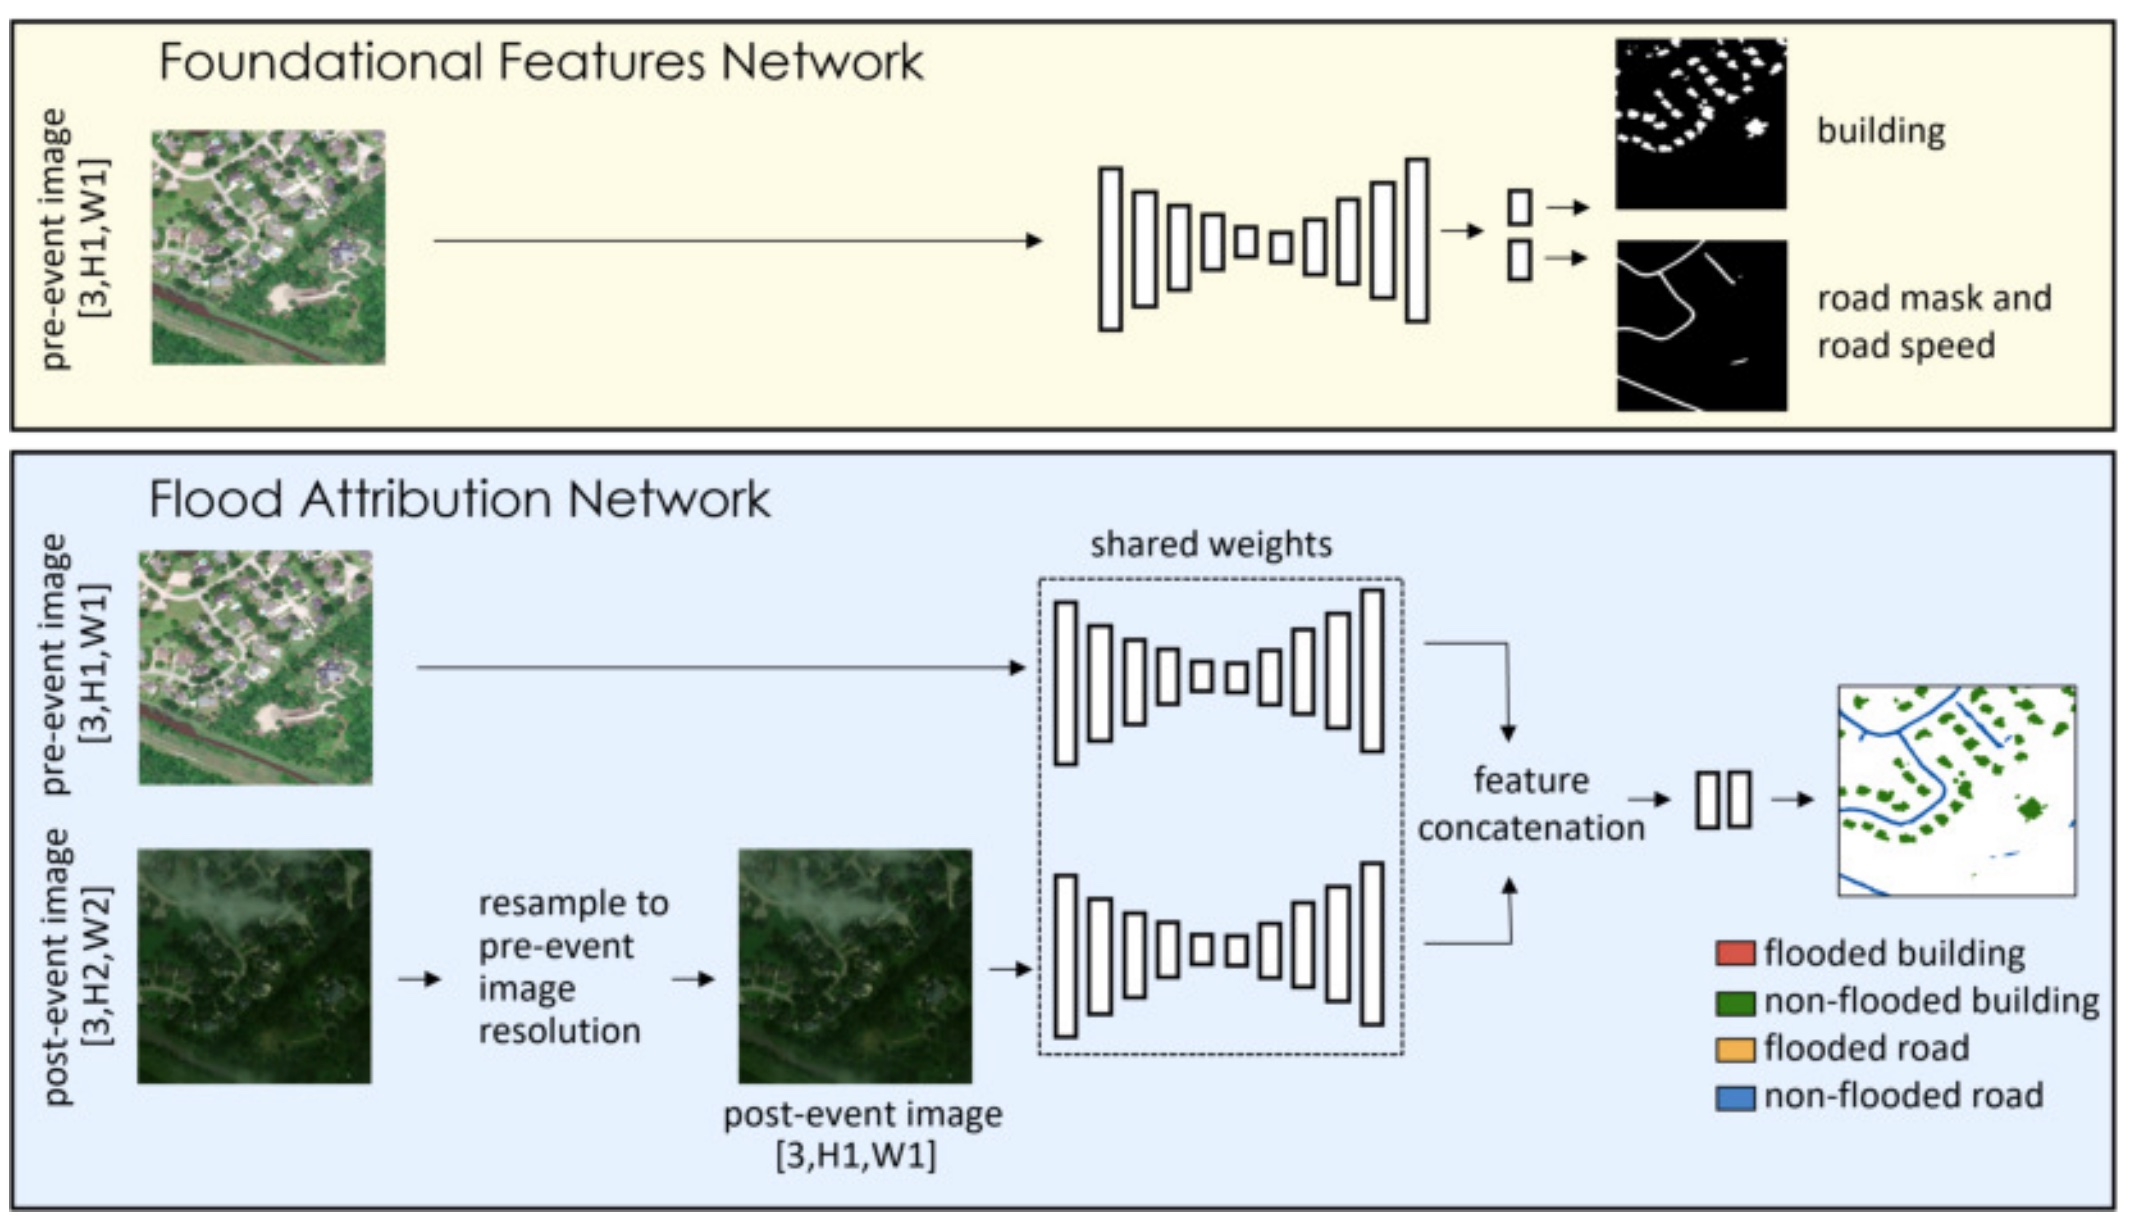
\includegraphics[width=1.0\linewidth]{figures/baseline.jpg}
   \caption{The foundation features network and flood attribution networks. The pipeline design is modular and allows different backbone models to be swapped in while maintaining the same data-loading, training, and evaluation code.}
   \label{fig:baseline}
\end{figure}



\subsection{SegFormer}
\begin{figure}[t]
  \centering
   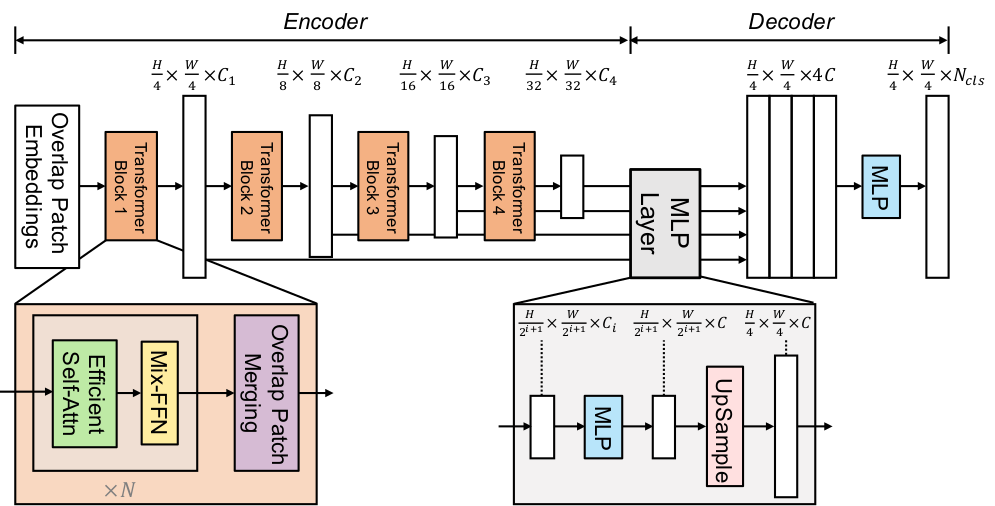
\includegraphics[width=1.0\linewidth]{figures/segformer_architecture.png}
   \caption{The Segformer model architecture has a transformer encoder and MLP decoder. The hierarchical structure is intended to capture multiple-scale features. Because the output reduces the Spatial dimension by a factor of 4, we add an upscaling layer to preserve image dimensions.}
   \label{fig:segformer}
\end{figure}

We experiment with increasingly large Segformer backbones to compare transformer based architectures with the baseline of CNNs. Segformer uses a hierarchical transformer encoder combining local and global attention to achive start-of-the-art performance on image segmentation tasks. Unlike ViT, Segformer does not use positional encoding which aids transfer learning between datasets with different image resolutions. This is important because the SpaceNet8 images have different resolutions than the images from the ImageNet, ADE20k, and Cityscale datasets used for pre-training.

We used Segformer b0, b1, and b2 models from the Huggingface transformers library \cite{wolf-etal-2020-transformers}. The difference between these variants is the number of parameters. We did not test the larger b3, b4, and b5 variants because they do not fit in the A6000 GPU's memory. Segformer reduces the spatial dimension by a factor of 4. We use nearest neighbor interpolation (\href{https://pytorch.org/docs/stable/generated/torch.nn.functional.interpolate.html}{link}) to upscale the segformer output to match the input spatial resolution. The models weights were initialized with pre-trained weights released by NVidia and each model was fine-tuned without freezing any parameters.

\subsection{DenseNet}
\begin{figure}[t]
  \centering
   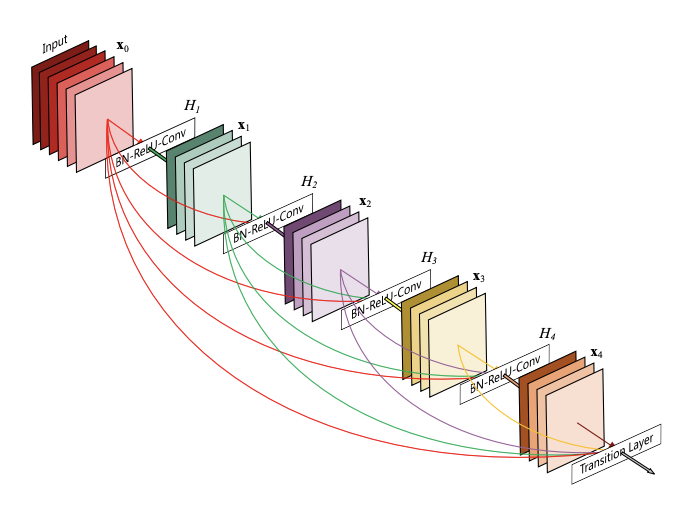
\includegraphics[width=0.8\linewidth]{final-report/figures/densenet1.png}
   \caption{DenseNet with 5 layers with expansion of 4}
   \label{fig:densenet}
\end{figure}

We experimented with DenseNet as one of the encoder structure for the U-net models. In traditional CNNs, the output of a layer is connected to the next layer after applying a series of operations, such as convolution, pooling, batch normalization, and an activation function. However, DenseNets differ in that they concatenate the output feature maps of a layer with the incoming feature maps, rather than summing them. To accommodate feature maps of different dimensions, DenseNets are divided into DenseBlocks, where the dimensions of the feature maps remain constant within each block, but the number of filters may vary towardsdatascience.com. To connect these DenseBlocks, transition layers are used, which handle operations such as downsampling and batch normalization. The advantage of DenseNet as stated in the original paper was that, as of the performance on ImageNet, it has similar performance as ResNet, but uses fewer than half as many parameters \cite{Huang2016DenselyCC}. We implemented DenseNet 121 and DenseNet 161 with weights pre-trained on ImageNet. The main difference between the 121 and 161 model is the size - DenseNet 121 is about 13MB in size while DenseNet 161 is about 100MB \cite{OpenVINO_DenseNet}.

\subsection{EfficientNet}
\begin{figure}[t]
  \centering
   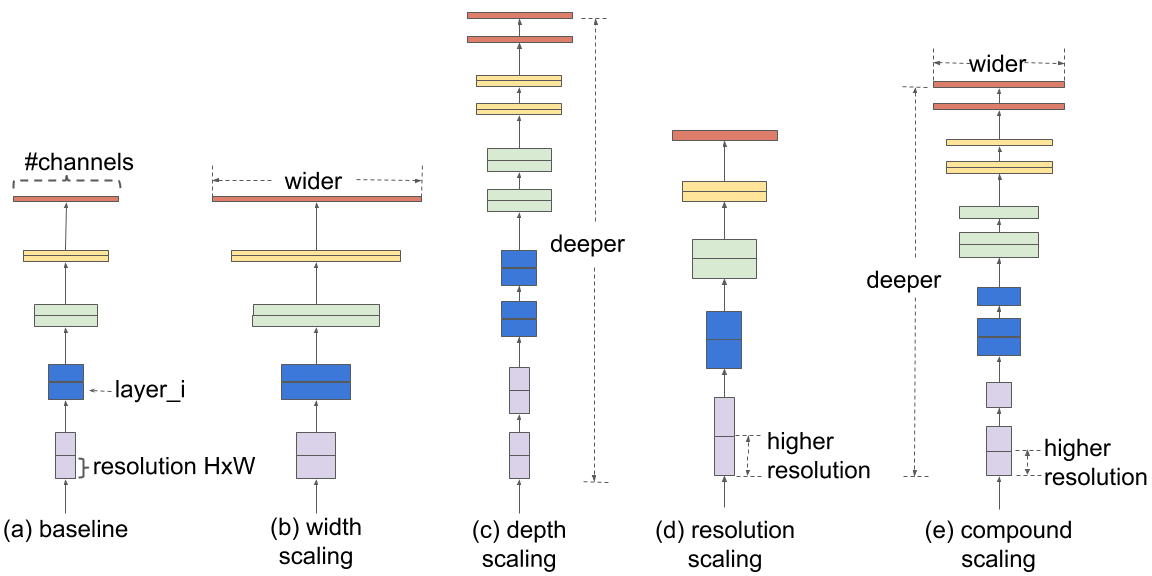
\includegraphics[width=0.8\linewidth]{final-report/figures/effnet.png}
   \caption{(a) Baseline network, (b)-(d) Conventional scaling, (e) Compound scaling in EfficientNet}
   \label{fig:effnet}
\end{figure}


Another encoder structure we experimented with was EfficientNet. The main difference between EfficientNet and traditional convolutional neural network is that EfficientNet uniformly scales all dimensions of depth/width/resolution using a compound coefficient. The advantage of EfficientNet is that it can generally achieve good accuracy on image classification tasks, such as ImageNet and transfer learning tasks, while requiring significantly fewer floating-point operations (FLOPs) for inference \cite{Keras_EfficientNet}. EfficientNet consists of a series of models (B0 to B7) that represent a good balance between efficiency and accuracy across different scales. We experimented with B2 and B4 models.


% Length: 2 pages

%Describe your learning algorithms, proposed algorithm(s), or theoretical proof(s). Make sure to include relevant mathematical notation, e.g. when you formulate your input(s), output(s) and the loss function(s). It is okay to use formulas from the lecture notes. For each algorithm, give a brief description (2-3 sentences) of how it works. Again, we are looking for your understanding of how these deep learning algorithms work. Although the teaching staff probably know the algorithms, future readers may not (reports will be posted on the class website). Additionally, if you are using a niche or cutting-edge algorithm (e.g. binary network, SURF features, or anything else not covered in the class), you may want to explain your algorithm using several paragraphs. Note: Theory/Algorithms projects may have an appendix showing extended proofs (see appendix description below). Assume the reader has completed CS231N. You don’t need to explain filters and max-pooling, but if you use something like stochastic strides, you should explain that.

%If you used an existing codebase and built on top of it, you must state this and explain what you wrote versus what the starter code already came with.



\section{Experiments}
\label{sec:experiments}

\subsection{SegFormer head}

The Segformer architecture (encoder-bottleneck-decoder) pre-trained on ImageNet produces a ($64, \frac{N}{4}, \frac{N}{4}$) mask and require a segmentation head to reduce the number of channels to 1 or 8 for the foundation features model and 4 for the flood attribution model.
To understand the model more, we have visualized the decoder output Fig. \ref{fig:segformer_decoder}. We experimented with three segmentation heads (single 1x1 convolution, single 3x3 convolution, and double 3x3 convolution). All work at this point was one using Segformer-b0. Loss and IoUs for all trials was similar; IoUs of $56.7\%$ (1x1 conv), $56.6\%$ (double 3x3), $57.1\%$ (3x3 conv) and we settled on a single 3x3 convolution layer. The training loss curves are shown in Fig. \ref{fig:segformer_head}.

\begin{figure}[t]
    \begin{center}
    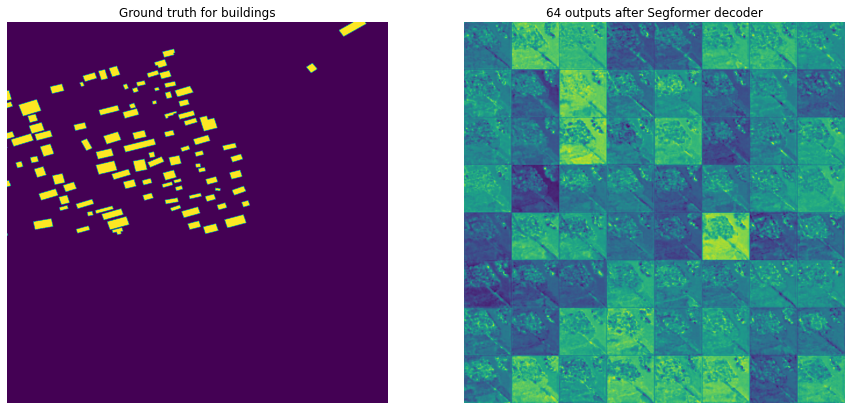
\includegraphics[width=\linewidth]{final-report/figures/decoder_output_layers.png}
    \caption{The left side shows the ground true segmentation mask for a group of buildings. The right sides shows an the Segformer decoder output for the image. The 64 output channels are arranged in a 8x8 grid of image blocks.}
    \label{fig:segformer_decoder}
    \end{center}
\end{figure}

\begin{figure}[t]
  \centering
   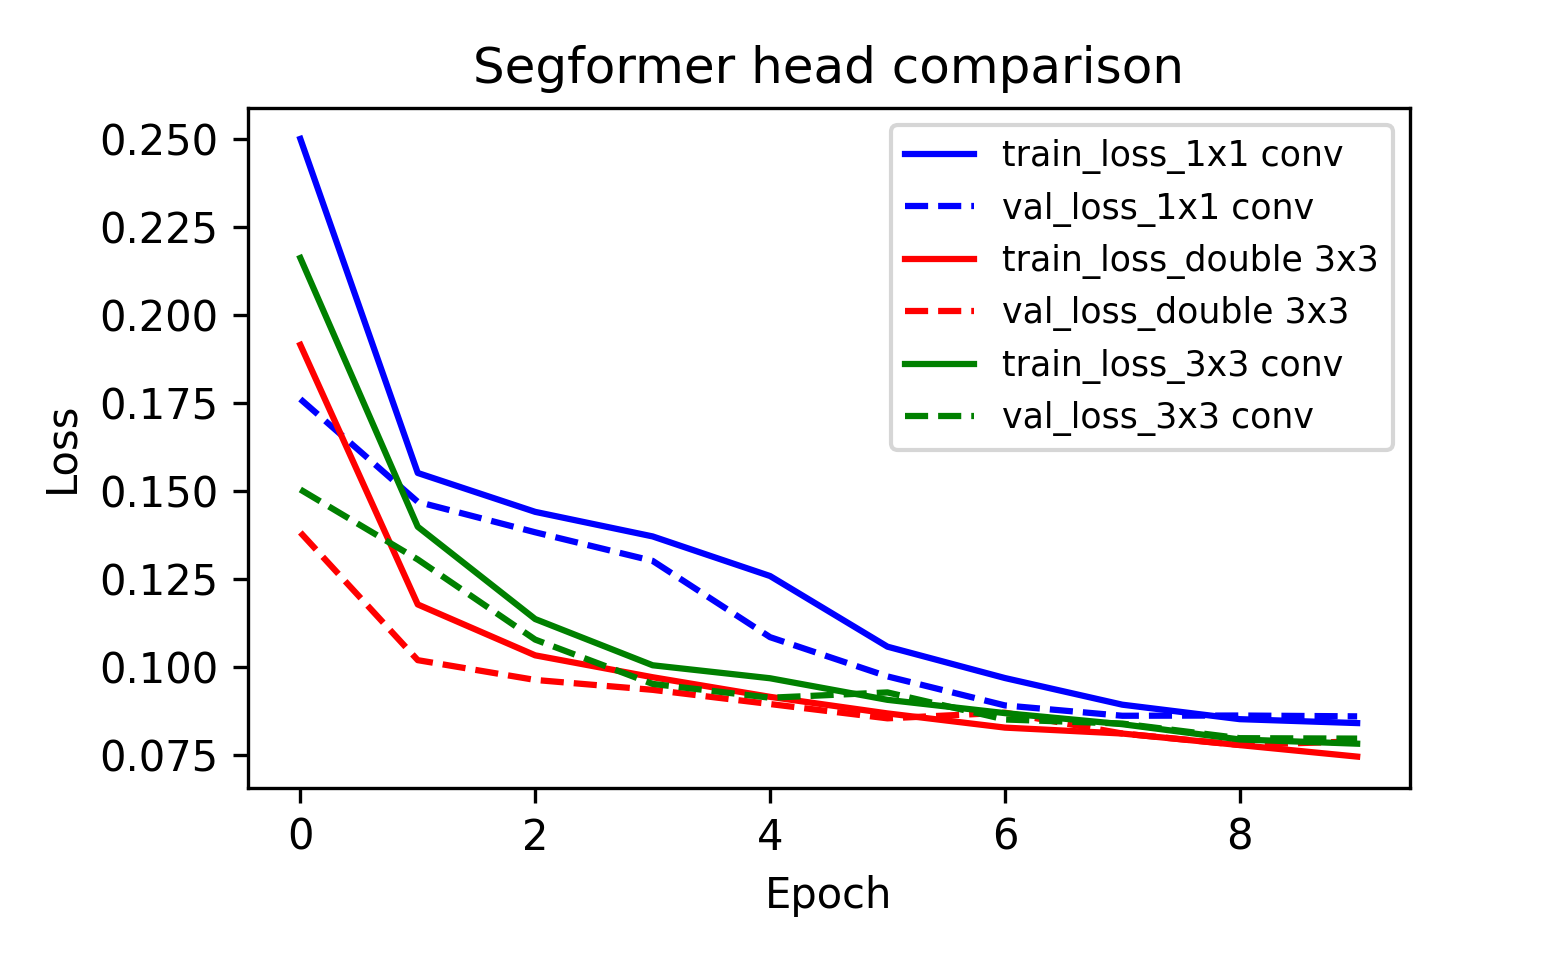
\includegraphics[width=1\linewidth]{figures/segformer_head_comparison.png}
   \caption{Loss for different Segformer segmentation heads were similar and we settled on a single 3x3 convolution layer.}
   \label{fig:segformer_head}
\end{figure}

\subsection{Pre-training}

We experimented with fine tuning models initialized from pre-trained weights. We observed a significant improvement in IoU for both Resnet34 and Segformer\_b0 flood and foundation feature networks (e.g. 0.56 IoU vs 0.36 IoU for the Resnet34 foundation features model). Additionally we compared pre-training the Segformer model on ImageNet, ADE20k, and Cityscapes datasets. The ImageNet dataset consists of images scraped from the internet of objects like animals, food, cars, etc \cite{ILSVRC15}. The ADE-20k dataset consists of annotated images with scenes of kitchens, bedrooms, stores, restaurants, etc \cite{zhou2017scene}. The Cityscapes dataset consists of annotated images of streets from 50 different cities \cite{cordts2016cityscapes}. We observe pre-training with ImageNet and Cityscapes yields an improvement over pre-training with ADE20k for the Foundation Features network and Flood network (See tables \ref{fig:pre-training-flood} and \ref{fig:pre-training-flood}). These results are expected because the outdoor images in the Cityscapes dataset are more similar to the SpaceNet8 dataset than the mostly indoor images from the ADE20k dataset.

An interesting observation is al the models are biased (higher IoUs) towards assigning not-flooded labels to buildings and roads. The worst case is the model fine-tuned from ADE20k weights which has zero IoU for flooded buildings and roads. This is due to the class imbalance in the SpaceNet8 dataset. Only 13\% of buildings and 15\% of roads are flooded. The flood network is trained using the cross-entropy loss function which does not adjust for the data imbalance. If we had more time we could use dice loss which is designed for highly unbalanced segmentation tasks. Even with the poor choice of loss function, the best Segformer model is still able to achieve reasonable IoUs for flooded roads and buildings.

\begin{table}
    \begin{tabular}{llll}
        Model (Pre-training) & Building IoU & Road IoU \\
        \hline
        Resnet34 (None) & 0.36 & 0.35 \\
        Resnet34 (Imagenet-1k) & 0.56 & \textbf{0.48} \\
        Segformer\_b0 (None) & 0.28 & 0.29 \\
        Segformer\_b0 (Imagenet-1k) & \textbf{0.59} & 0.47 \\
        Segformer\_b0 (ADE20k) & 0.54 & 0.44 \\
        Segformer\_b0 (Cityscapes) & 0.58 & 0.47 \\
    \end{tabular}
    \caption{Comparison of pre-trained vs not pre-trained Foundation Features networks. The best IoUs for Building and Road segment are in bold. Pre-training provides a 0.13 to 0.31 increase in IoU.}
    \label{fig:pre-training-foundation}
\end{table}

\begin{table}
    \begin{tabular}{lllll}
        Model (Pre-training) & \makecell{NF \\ Bldg} & \makecell{F \\ Bldg} & \makecell{NF \\ Road} & \makecell{F \\ Road} \\
        \hline
        Resnet (None) & 0.28 & 0.03 & 0.10 & 0.00 \\
        Resnet (Imagenet) & 0.46 & 0.12 & 0.30 & 0.18 \\
        Segformer (None) & 0.22 & 0.01 & 0.13 & 0.00 \\
        Segformer (Imagenet) & 0.58 & 0.38 & \textbf{0.43} & \textbf{0.37} \\
        Segformer (ADE20k) & 0.46 & 0.0 & 0.31 & 0.03 \\
        Segformer (Cityscapes) & \textbf{0.61} & \textbf{0.40} & 0.41 & 0.34 \\
    \end{tabular}
    \caption{Comparison of pre-trained vs not pre-trained Flood networks. Pre-training the Segformer model on the Cityscapes dataset provides a 0.39 increase in IoU for both Not-Flooded Building (NF Bldg) and Flooded Building (F Bldg) classes and Pre-training on ImageNet provides similar increase for Road segmentation.}
    \label{fig:pre-training-flood}
\end{table}

\subsection{Compute Resource Analysis}

All of our computations were done on the Paperspace platform initially using P6000 GPUs, and later A6000. In order to understand hardware limitations we studied some of the GPU components across different models, chiefly: space and time complexity in the form of memory consumption and epoch duration respectively. As expected we observed large differences among models. 

\begin{figure}[t]
  \centering
   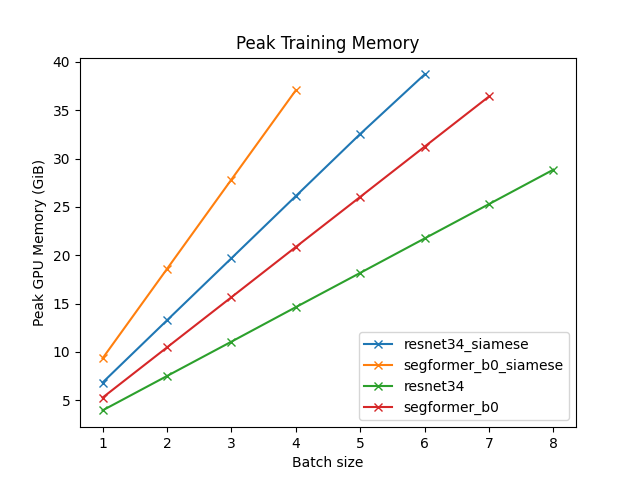
\includegraphics[width=1.0\linewidth]{final-report/figures/peak_training_gpu_memory.png}
   \caption{Peak GPU memory consumption for different models and different batch sizes.}
   \label{fig:peak_gpu_memory}
\end{figure}

We measured the peak GPU memory consumed by each model for various batch sizes because GPU memory constrained the size of the Segformer models we could train on the A6000 GPU. The y-intercept of the memory vs batch-size best fit line is the memory from model weights, their gradients, and overhead. The slope represents the memory for training examples, activations, and gradients of activations. The Siamese networks consume almost twice as much memory for a given batch sizes because they operate on two images per training-example vs a single image per training-example for the Foundation features network. Additionally we observe Segformer\_b0 consumes more memory that Resnet34 despite having fewer parameters which can be described by fundamentally different calculation done by attention vs convolution. Indeed, another difference between CNN vs Transformed based models can be seen in epoch duration (Figure \ref{fig:epoch_time}). Segformer (b0, b1, b2) all have longer epochs even though they have fewer parameters. This is not surprising considering attention has quadratic complexity in comparison to CNN linear. (Transformer time complexity is $O(n^2d + nd^2)$ where n is the number of image patches and d is the size of the vector representations. (n,d) are dimensions of query, key, and value matrices in self-attention).

\begin{figure}[t]
  \centering
   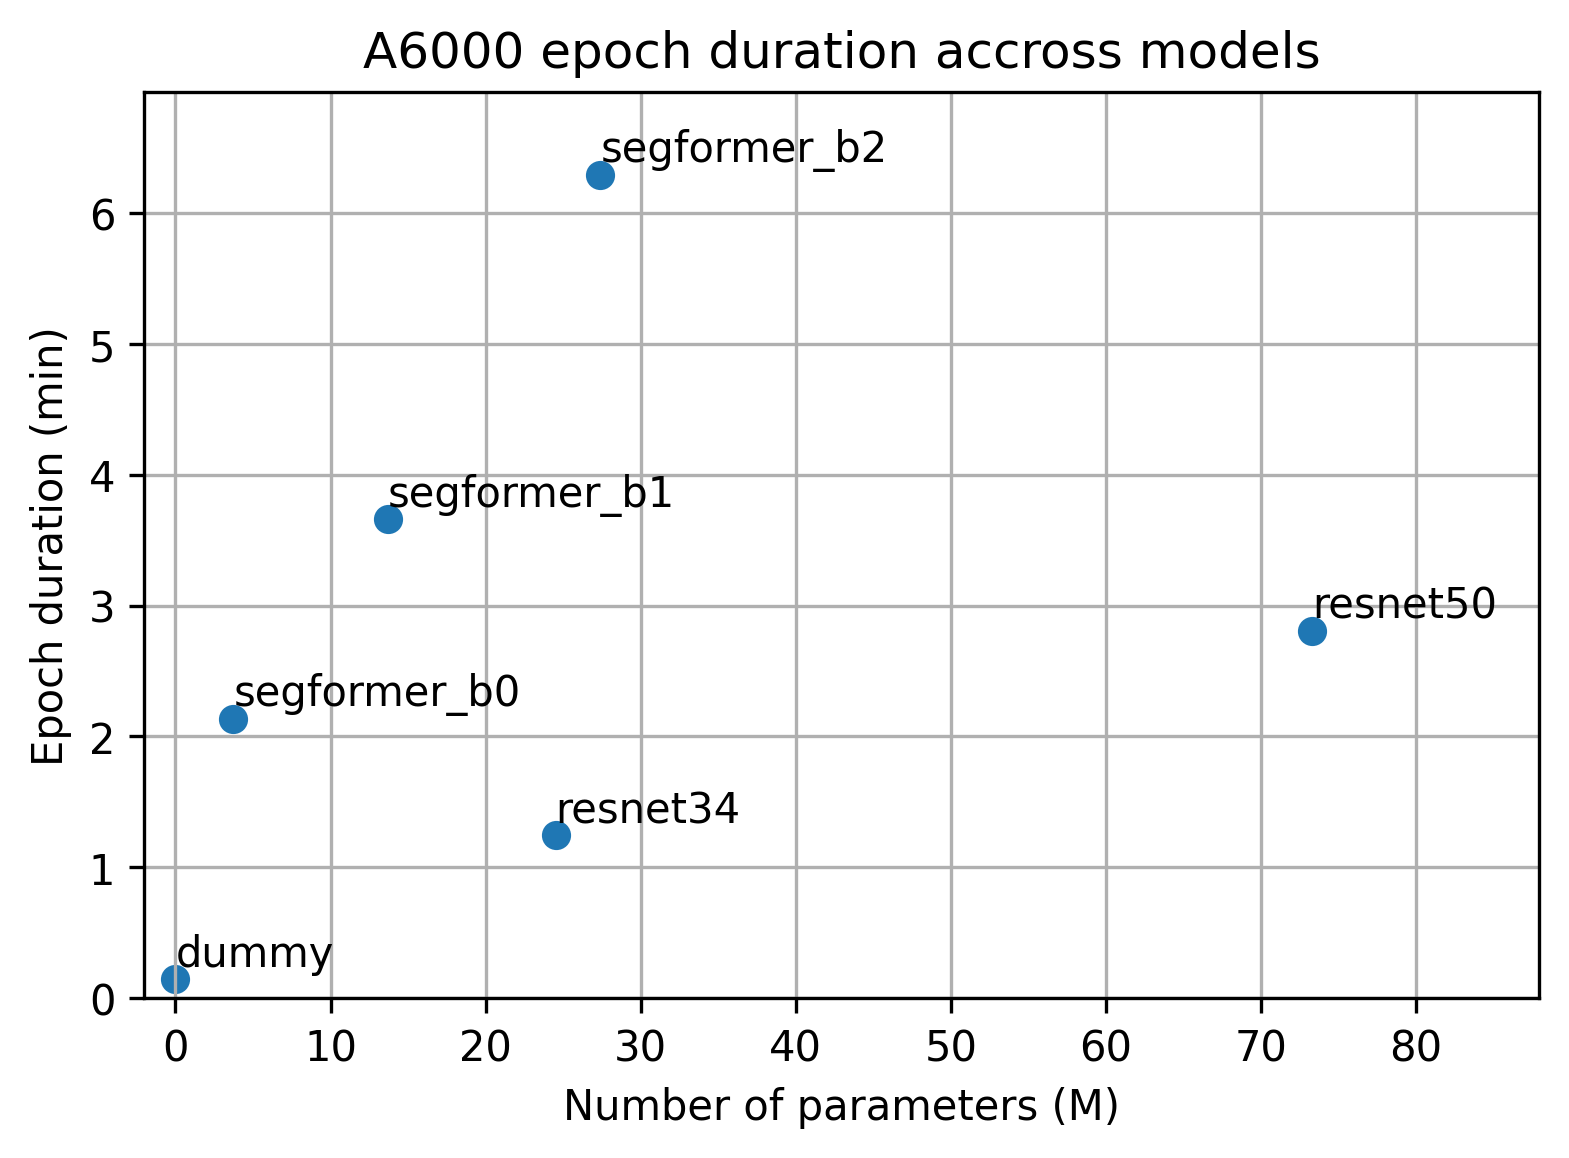
\includegraphics[width=0.9\linewidth]{figures/epoch_time.png}
   \caption{Total epoch duration on the A6000 GPU compared with the number of parameters for each model. As a baseline we trained a dummy model consisting of a single 1x1 conv layer projecting from the input to output dimension.}
   \label{fig:epoch_time}
\end{figure}

We also noticed one particular quirk regarding data loading from hard drive into CPU RAM, namely, the difference between using shared network drive and local hard drive. For quite some time we have employed a shared network drive for all of our data storage to facilitate working on multiple instances. Typical epoch would take 4.5 minutes regardless of the model we were testing. This was a surprising result and we initially assumed that the bottleneck was in the amount of time it takes to transfer data from CPU to GPU memory. The truth was different, and follow up experiment of loading data from a local hard drive cut the training time of Resnet34 3-fold. A stark 6.5X difference in data loading speed from shared network drive (4 minutes) vs local hard drive (40 seconds) was causing data loading to be computational bottleneck for all but Segformer\_b2 model (considering CPU data loading and GPU computation happen in parallel). It is a cautionary tale that we will keep in mind when training future models.

\subsection{Model comparison}

We finally compare IoUs and number of parameters across all models (Figure \ref{fig:iou_vs_model}). While most models performed similarly when detecting buildings in pre-event images, Segformer\_b1 and b2  emerged as much better option when detecting flooded buildings (~40\%) vs others (Table \ref{fig:pre-training-flood}). Qualitatively Segformer is noticeably better at detecting polygonal shapes with sharp edges vs blob-like structures detected by CNN based models. This can be explained as another attention advantage over CNN. For qualitative comparison refer to Figures \ref{fig:sample_images_foundation_0}-\ref{fig:sample_images_flood_2} in Appendix.

\begin{figure}[t]
  \centering
   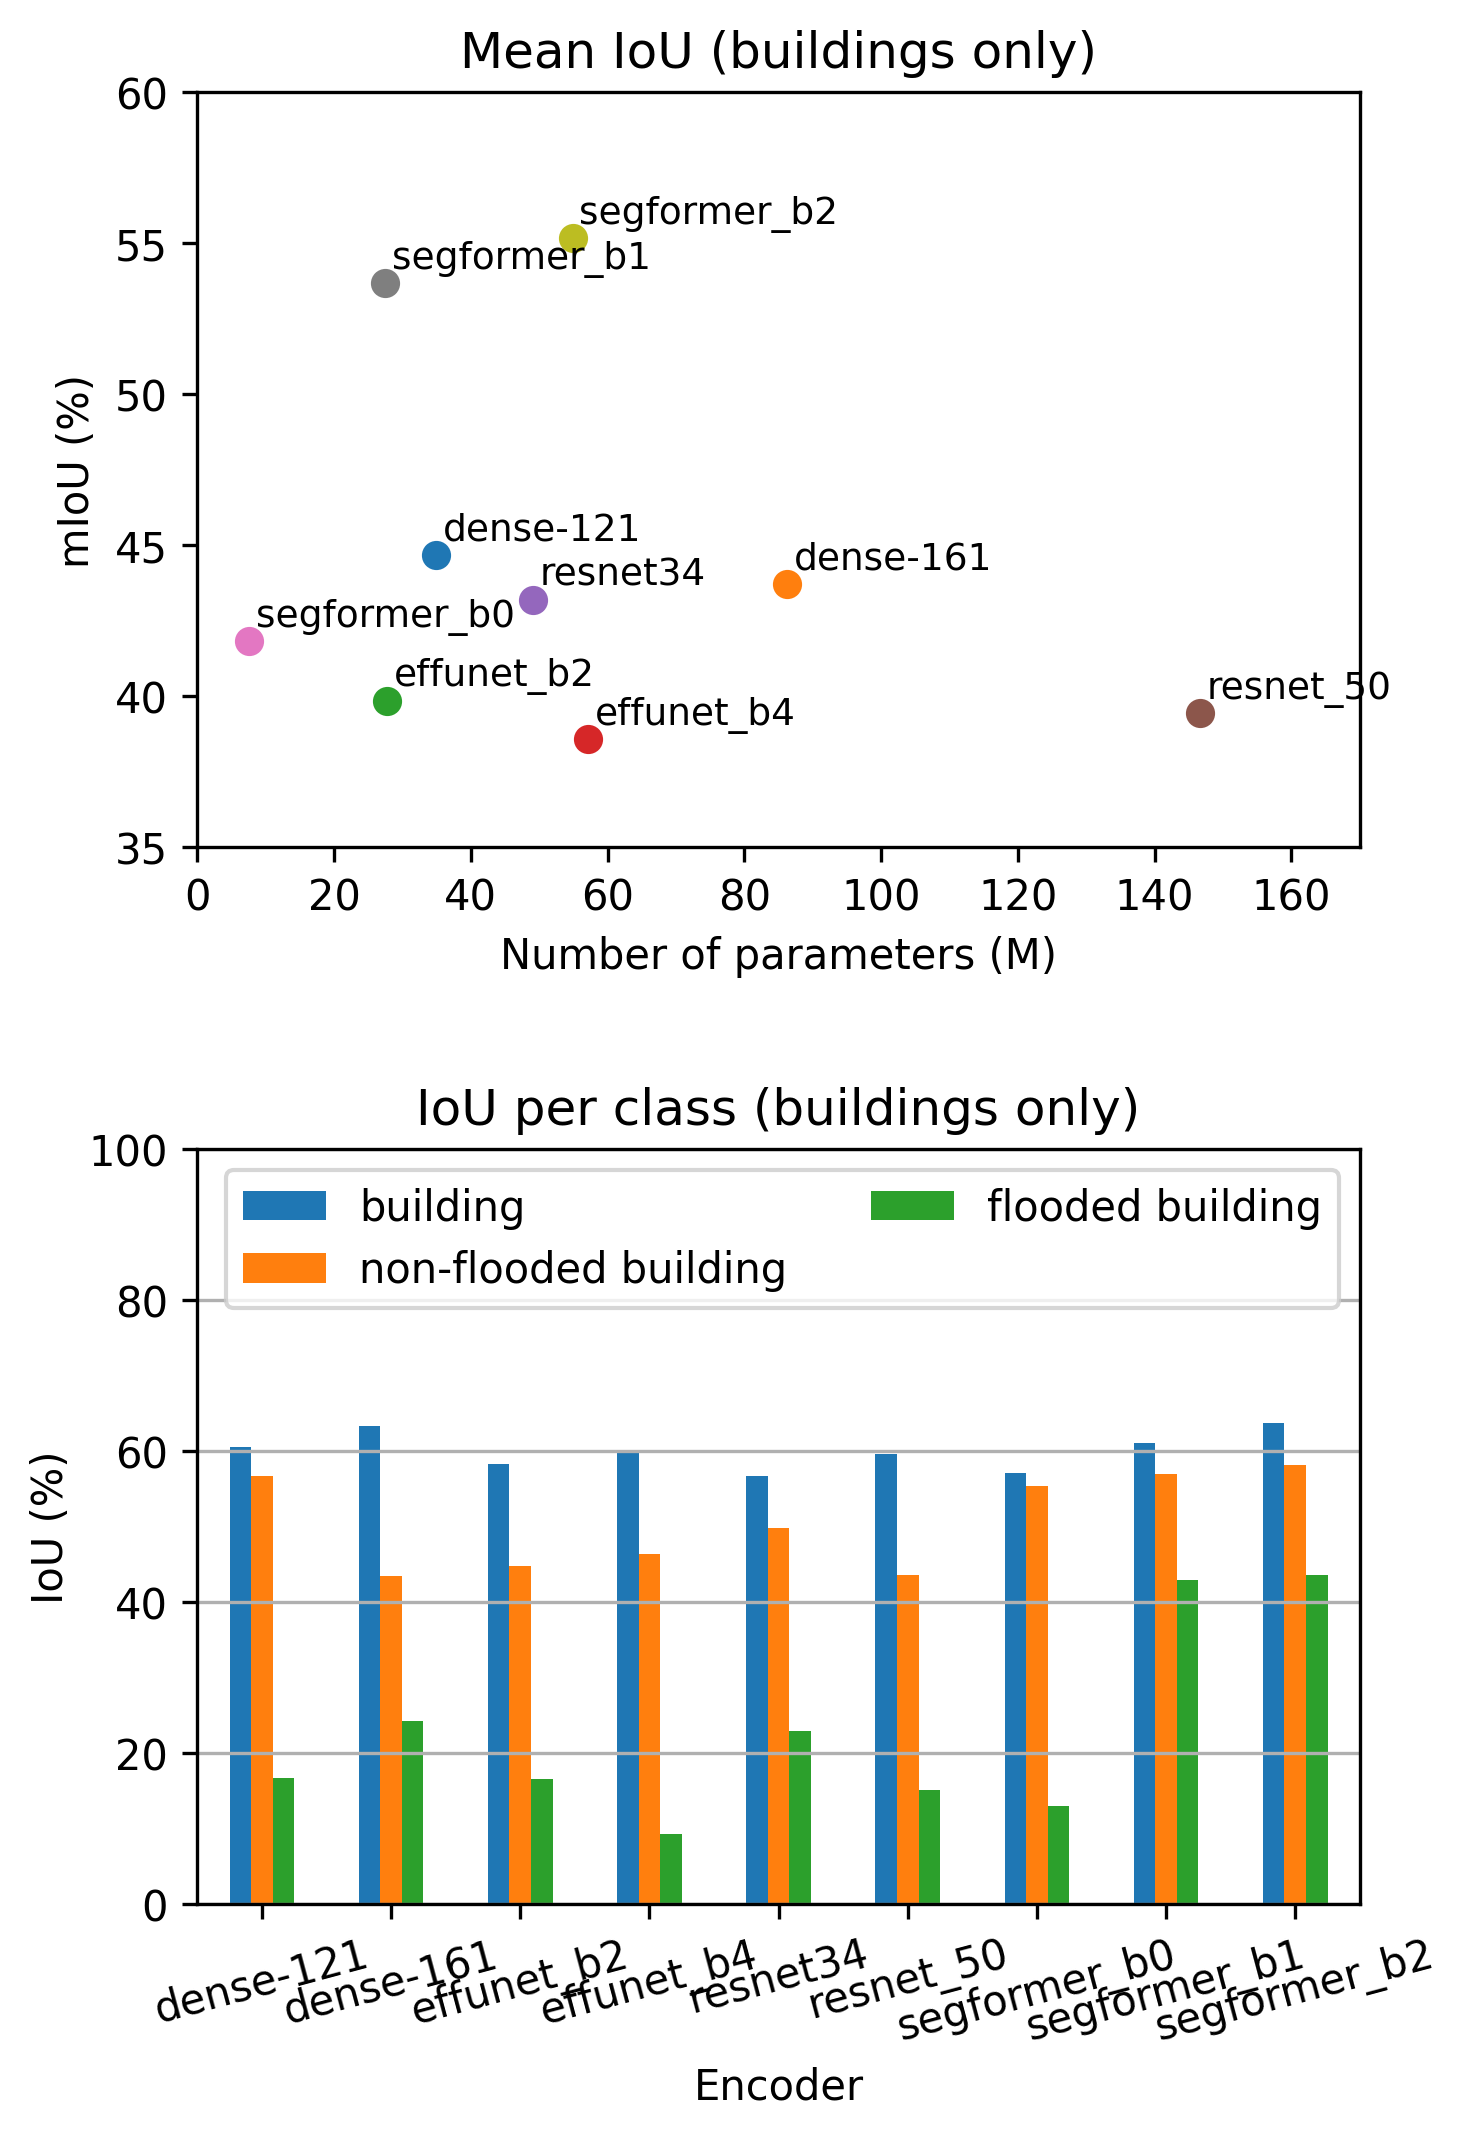
\includegraphics[width=1.1\linewidth]{figures/iou_vs_model.png}
   \caption{IoU comparison between models for building detection only. Segformer models outperform CNN based one, showing that attention is better suited for detecting building and road-like polygonal objects.}
   \label{fig:iou_vs_model}
\end{figure}

\section{Discussion}
\label{sec:discussion}

%You should also briefly give details about what hyperparameters you chose (e.g. why did you use X learning rate for gradient descent, which optimizer did you pick, what was your mini-batch size and why) and how you chose them. Did you do cross-validation, and if so, how many folds? This should not take more than 1-2 paragraphs. If you want to list more details, please do so in the supplemental material.

%Before you list your results, make sure to list and explain what your primary metrics are: accuracy, mAP, inception/mode scores, etc. Provide equations for the metrics if necessary.

%For results, you want to have a mixture of tables and plots. Both quantitative and qualitative results are necessary. To reiterate, you must have both quantitative and qualitative results! This includes unsupervised learning (talk with the TAs on how to quantify unsupervised methods). Include visualizations of results, heatmaps, saliency maps, examples of failure cases and a discussion of why certain algorithms failed or succeeded. 

We have used early-stopping for all models (roughly 10 epochs) where validation loss would plateau. We did notice overfitting on training dataset ($>10$ epochs) that could be explained with the fact that all models have large amount of parameters (in the millions) while there are only hundreds of training images (adding more training data would have helped of course). However, since we didn't observe directly overfitting on a validation dataset we consider that all models generalized well.

Road detection seems to have been much harder then building detection. Qualitatively, road have been detected especially in the pre-event images. It is possible that IoU might not be the best metric when it comes to road detection considering it's elongated shape. It is possible that misalignment of the pre- and post-images could have caused whole roads to be missed. We admit improvement can be done to this end (SpaceNet3 dataset was particularly designed for read detection and can serve for further inspiration).

%Here’s a list of qualitative \& quantitative methods for analysis that might be helpful in your project. None of these are necessary nor will be explicitly looked for by graders – rather, we wanted to provide some (non-exhaustive) guidance on analysis methods:


\section{Conclusion/Future Work}
\label{sec:conclusion}


% TODO:
% \begin{itemize}
%     % \item In conclusion we find large pre-trained Segformer models are higher performing that Resnet and U-net based models
%     % \item We think the pre-trained models performed better than training from scratch because we were only able to train for a relatively small number of epochs (e.g. 10) on a small dataset of ~700 images. With a larger dataset and more more epochs the advantage from pre-training would shrink.
%     % \item Future work includes normalizing images or applying other preprocessing techniques, pre-training on additional data (e.g. building and road network datasets from previous SpaceNet challenges), and combining models into ensembles (e.g. pre-training on ImageNet is better for road segmentation while pre-training on Cityscapes is better for flooded building segmentation). Additionally we should change the loss function for the flood network from cross-entropy to one that accounts for class imbalances.
%     \item Additional models
% \end{itemize}

In conclusion, we found that large pre-trained Segformer models outperformed Resnet and U-net based models. We hypothesize that the pre-trained models performed better because we only trained for a relatively small number of epochs on a small dataset of 700 images. With a larger dataset and more epochs, the advantage from pre-training would shrink. Additionally, different convolution layers were tested for the segmentation head, with similar IoUs of 56.7\% (1x1 conv), 56.6\% (double 3x3), and 57.1\% (3x3 conv), ultimately settling on a single 3x3 convolution layer. This project also compared memory consumption and epoch duration across different models, observing that SegFormer models consume more memory and have longer epochs despite having fewer parameters compared to ResNet34. We reasoned that attention has quadratic complexity, contributing to the longer epoch durations for SegFormer models. Another interesting observation was the impact of data loading from a network attached storage versus a local hard drive. Loading data from a local hard drive took only 40 seconds, while loading from a shared drive took 4.5 minutes, resulting in a 6x speedup when using a local hard drive. This difference in data loading time highlights the importance of data storage and access methods when working with computationally intensive models like SegFormer.

As for future work, we propose to implement several techniques to improve the segmentation accuracy of our deep learning model. First, we will normalize images and apply other pre-processing techniques to reduce variance and improve model convergence. Second, we will pre-train the model on additional datasets, such as building and road network datasets from previous SpaceNet challenges, to improve its ability to recognize different features in satellite images. Since we observed that different models could have different performance in specific segmentation task - for example, pre-training on ImageNet is better for road segmentation, while pre-training on Cityscapes is better for flooded building segmentation - we could also combine models into ensembles to improve the performance. Finally, we will change the loss function for the flood network from cross-entropy to one that accounts for class imbalances to improve accuracy in the segmentation of flooded buildings. 
In addition to the potential work we can do with our existing models, there are a few different model architectures that we can explore. We tried the state-of-art model Segment Anything (SAM) on our image. The model was able to segment the image neatly into different parts but the segmentation was too granulated and was not suitable for our application (\ref{fig:sam}) - for example the trees on the field was segmented but a road was missed. This result is in fact not bad given that it is zero-shot. In the future we could try to fine-tune this model so that if focuses on the specific instances we want and gives better performance for our tasks. 


\begin{figure}[t]
  \begin{center}
  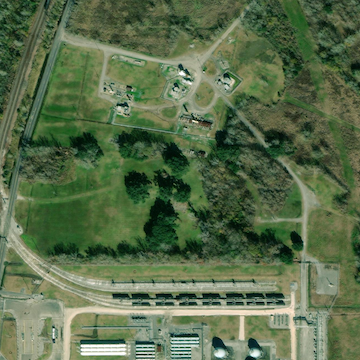
\includegraphics[width=0.48\linewidth]{final-report/figures/SAM_example.png}
   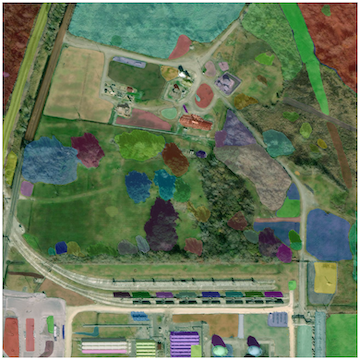
\includegraphics[width=0.48\linewidth]{final-report/figures/SAM_example_eval.png}
   \caption{Example of Segment Anything prediction with zero-shot learning on satellite images. Fine-tuning it could be a next promising step.}
   \label{fig:sam}
  \end{center}
   
\end{figure}


% Length: 1-3 paragraphs

%Summarize your report and reiterate key points. Which algorithms were the highest-performing? Why do you think that some algorithms worked better than others? For future work, if you had more time, more team members, or more compute, what would you explore?

%All the text in sections before this point must fit on eight (8) CVPR-style pages or less. Extra figures can go beyond the limit, but please do not put all your figures at the end just to fit the page limit. TAs will also be focusing their attention largely on the previous sections, so anything critical to your project should go in those sections, if possible. (If you are unsure of something, please feel free to make a private Ed post).

%This section is optional. Include additional derivations of proofs which weren’t core to the understanding of your proposed algorithm. Usually, you put equations or other details here when you don’t want to disrupt the flow of the main paper.

\section{Contributions \& Acknowledgements}
\label{sec:contributions}

We made the following contributions and utilized the following GitHub repositories:
\begin{itemize}
    \item Adrian: Segformer model integration, peak-GPU memory measurements, pre-trained vs not pre-trained experiments.
    \item Naijing: EfficientNet and Densenet model integrations.
    \item Nenad: IoU vs number of parameters measurements, segment anything, Segformer head comparison, epoch runtime comparison.
    \item Repositories: \href{https://github.com/SpaceNetChallenge/SpaceNet8}{SpaceNet8 baseline pipeline}, \href{https://github.com/huggingface/transformers/releases}{Segformer model}, \href{https://github.com/LovreAB17/Eff-UNet}{EfficientNet model}, \href{https://github.com/facebookresearch/segment-anything}{Segment Anything}, \href{https://github.com/liuzhuang13/DenseNet}{DenseNet}, \href{https://github.com/motokimura/spacenet8_solution_5th-place/tree/main/spacenet8_model/models}{5th place SpaceNet8 Challenge Entry}.
\end{itemize}

%In this section, you must explicitly state what each person on your team did for the project. If you made use of public code (e.g. from GitHub), please provide a link to the original repo. Additionally, you must mention any non-CS231N collaborators and include a brief sentence on what they did for your project. See the \href{https://www.nature.com/articles/nature16961#author-information}{AlphaGo paper’s contributions statement} for an example. If you’re part of a research lab and made use of their job scheduling, containerization, or GPUs, briefly include a sentence description on this as well.

\pagebreak
\section{References/Bibliography}

%This section should include citations for: (1) Any papers mentioned in the related work section. (2) Papers describing algorithms that you used which were not covered in class. (3) Code or libraries you downloaded and used. This includes libraries such as scikit-learn, TensorFlow, PyTorch, etc. For simplicity, please use the provided BibTeX file in the template (see our "Section 2" suggestions for how to easily get BibTeX citations from Google Scholar). Main body text, figures, and any discussions are strictly forbidden from this section. We are excluding the references section from the page limit to encourage students to perform a thorough literature review/related work section without being space-penalized if they include more references.

%%%%%%%%% REFERENCES



{\small
\bibliographystyle{ieee_fullname}
\bibliography{egbib}
}

\section{Appendix}
\label{sec:appendices}

\clearpage
\begin{figure}[t]
  \centering
   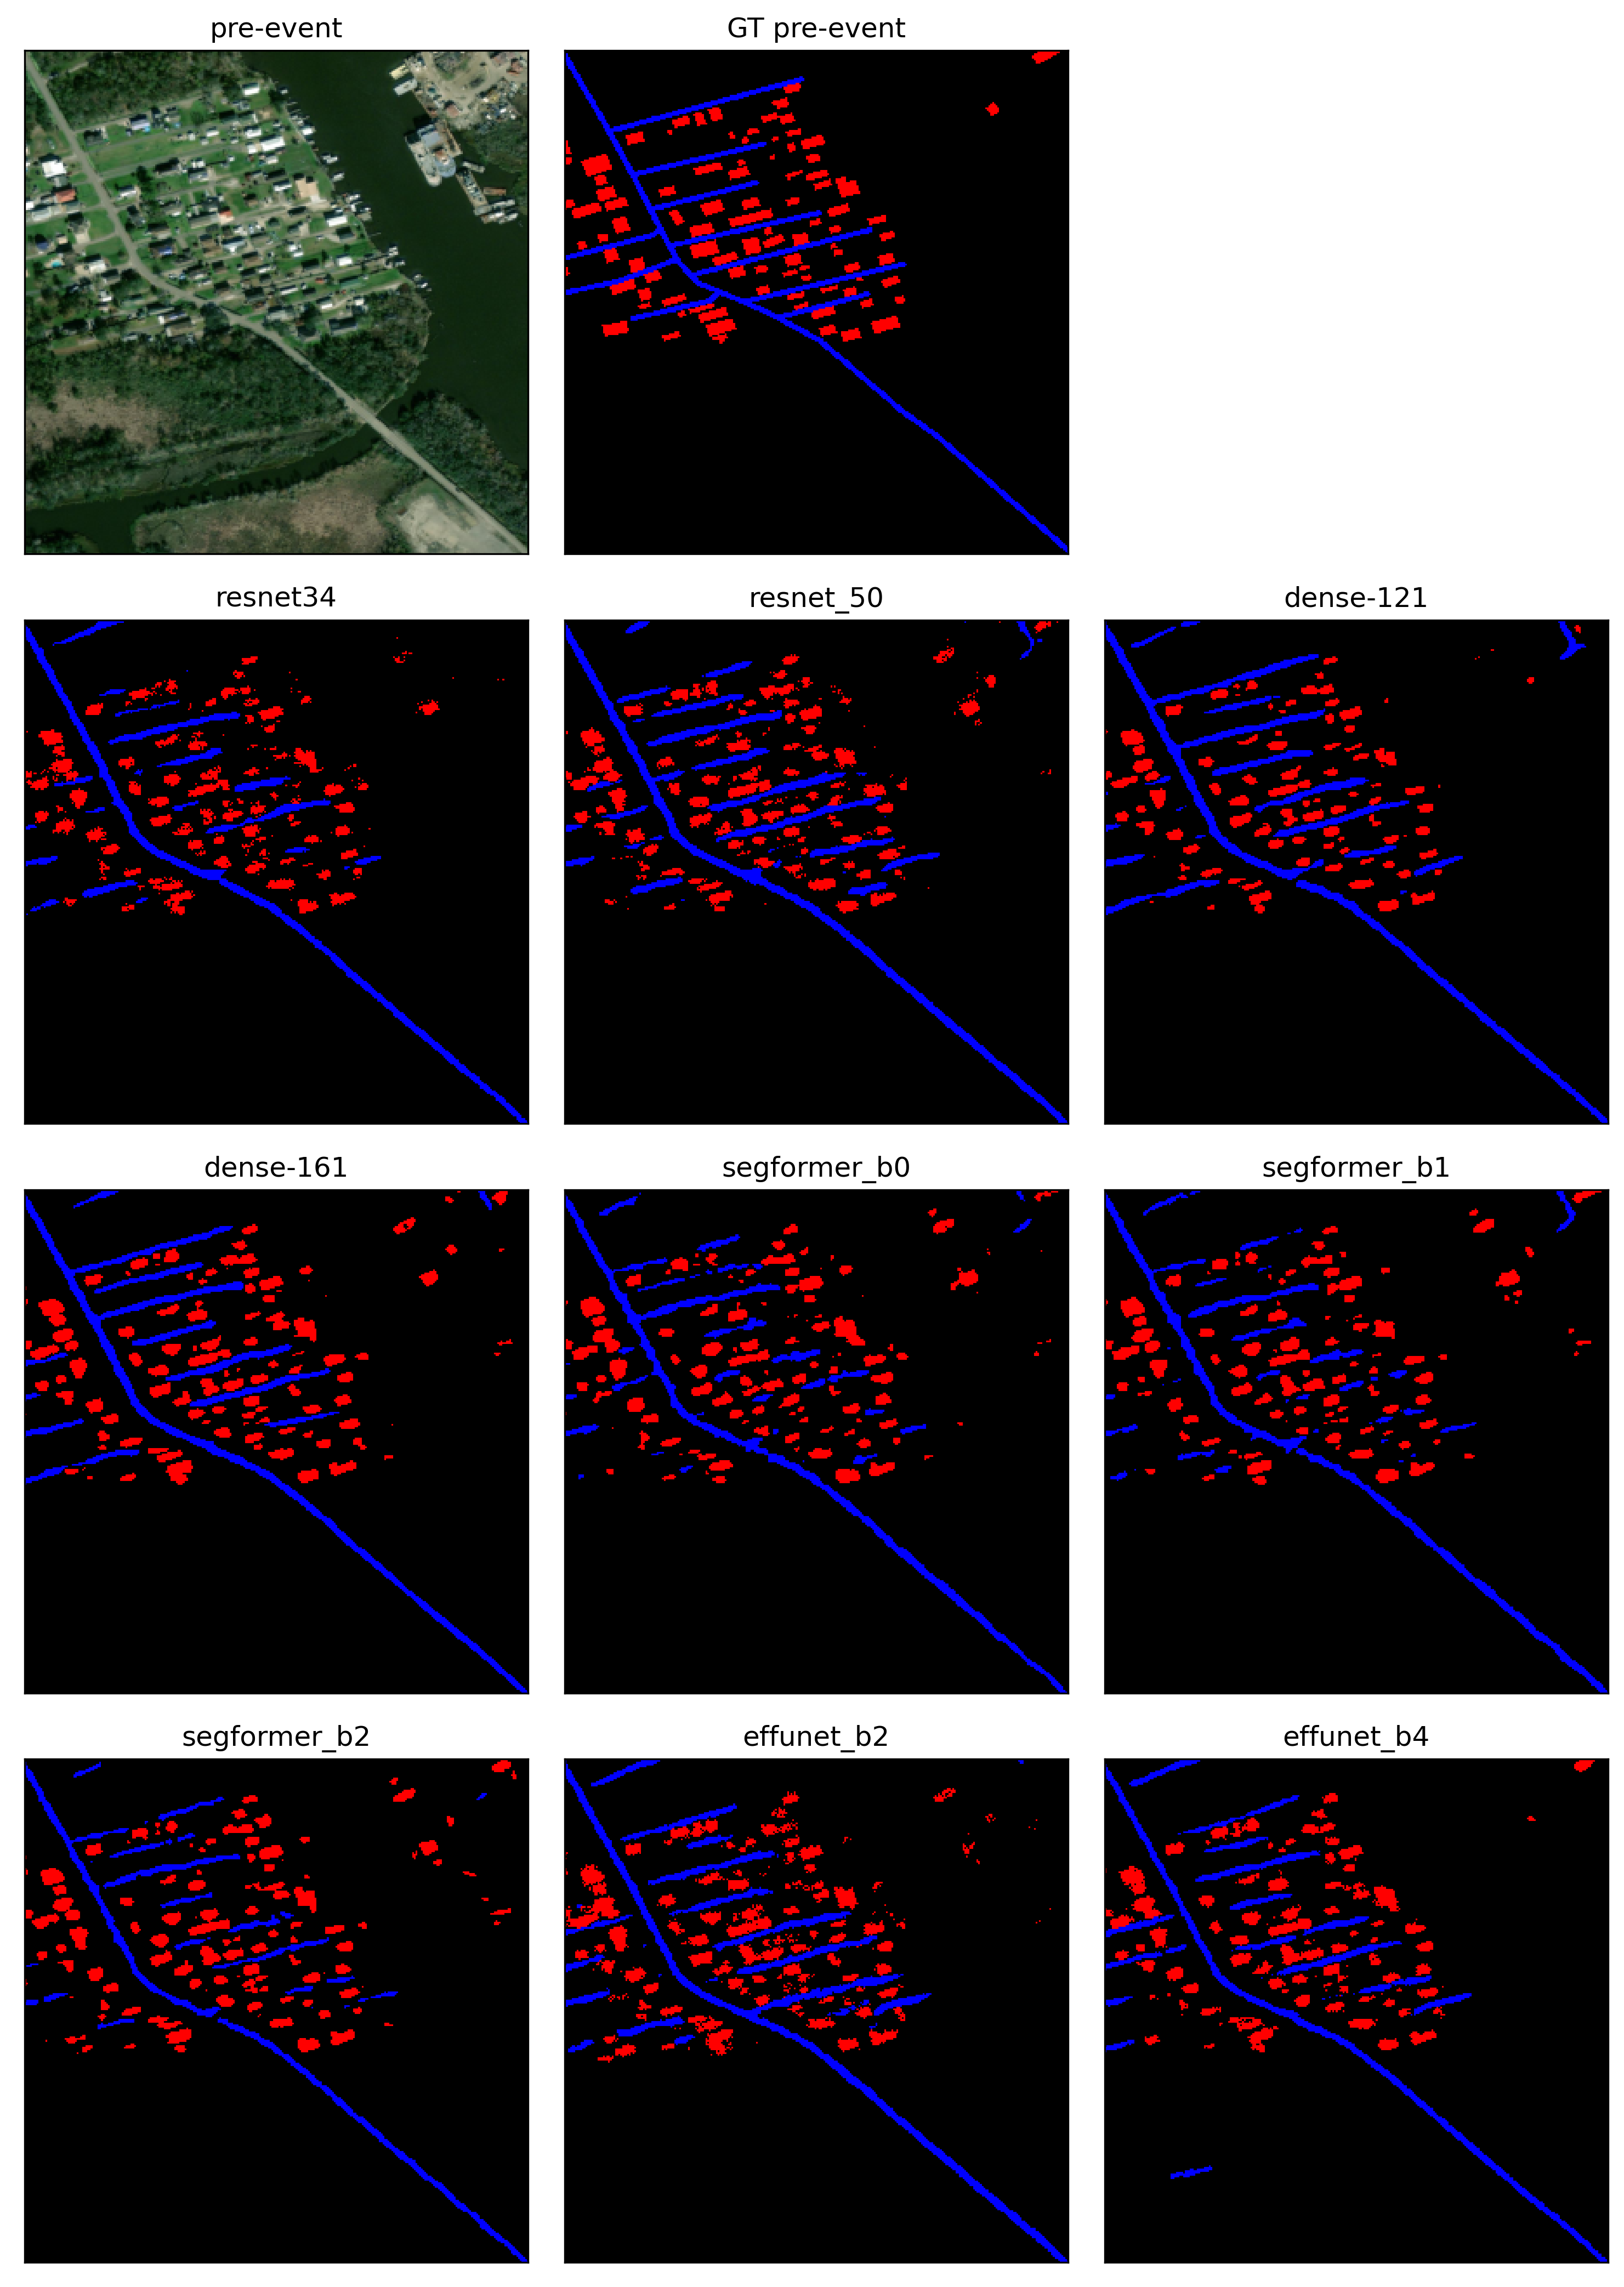
\includegraphics[width=2\linewidth]{final-report/figures/sample_images_foundation_0.png}
   \caption{Predictions across Foundation network models.}
   \label{fig:sample_images_foundation_0}
\end{figure}

\clearpage
\begin{figure}[t]
 \centering
  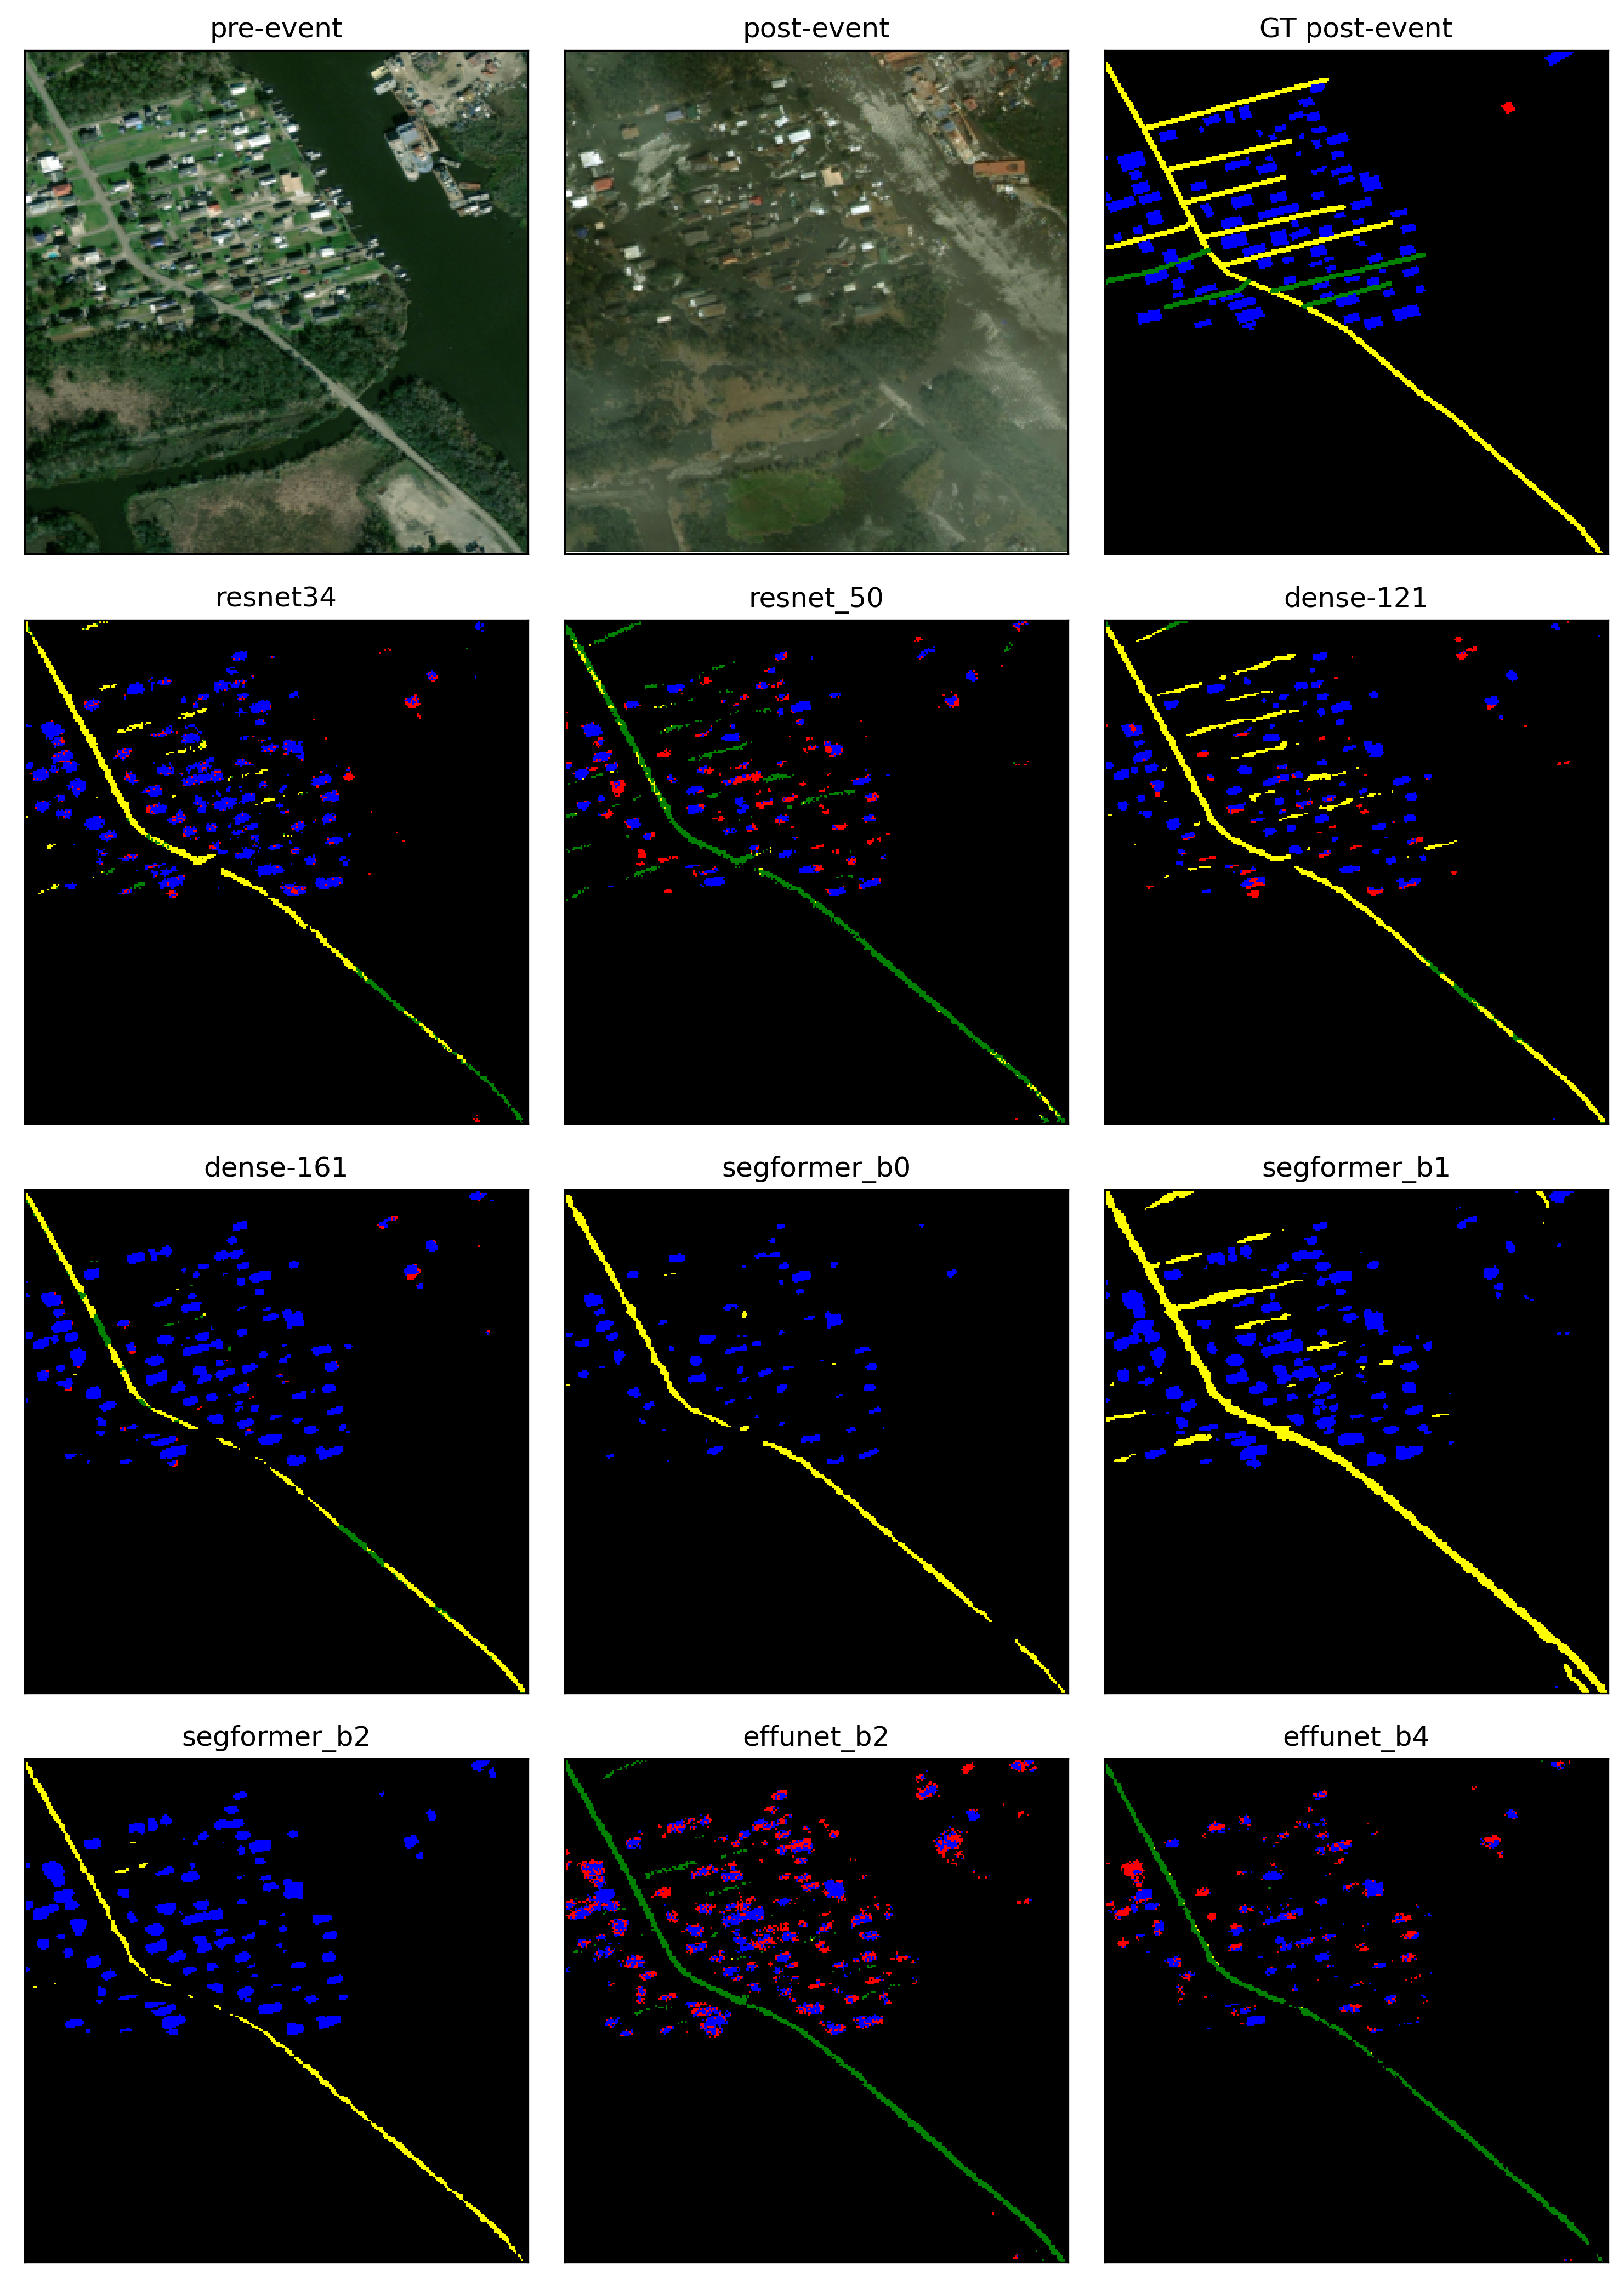
\includegraphics[width=2\linewidth]{final-report/figures/sample_images_flood_0.png}
  \caption{Predictions across Flood network models.}
  \label{fig:sample_images_flood_0}
\end{figure}


\clearpage
\begin{figure}[t]
  \centering
   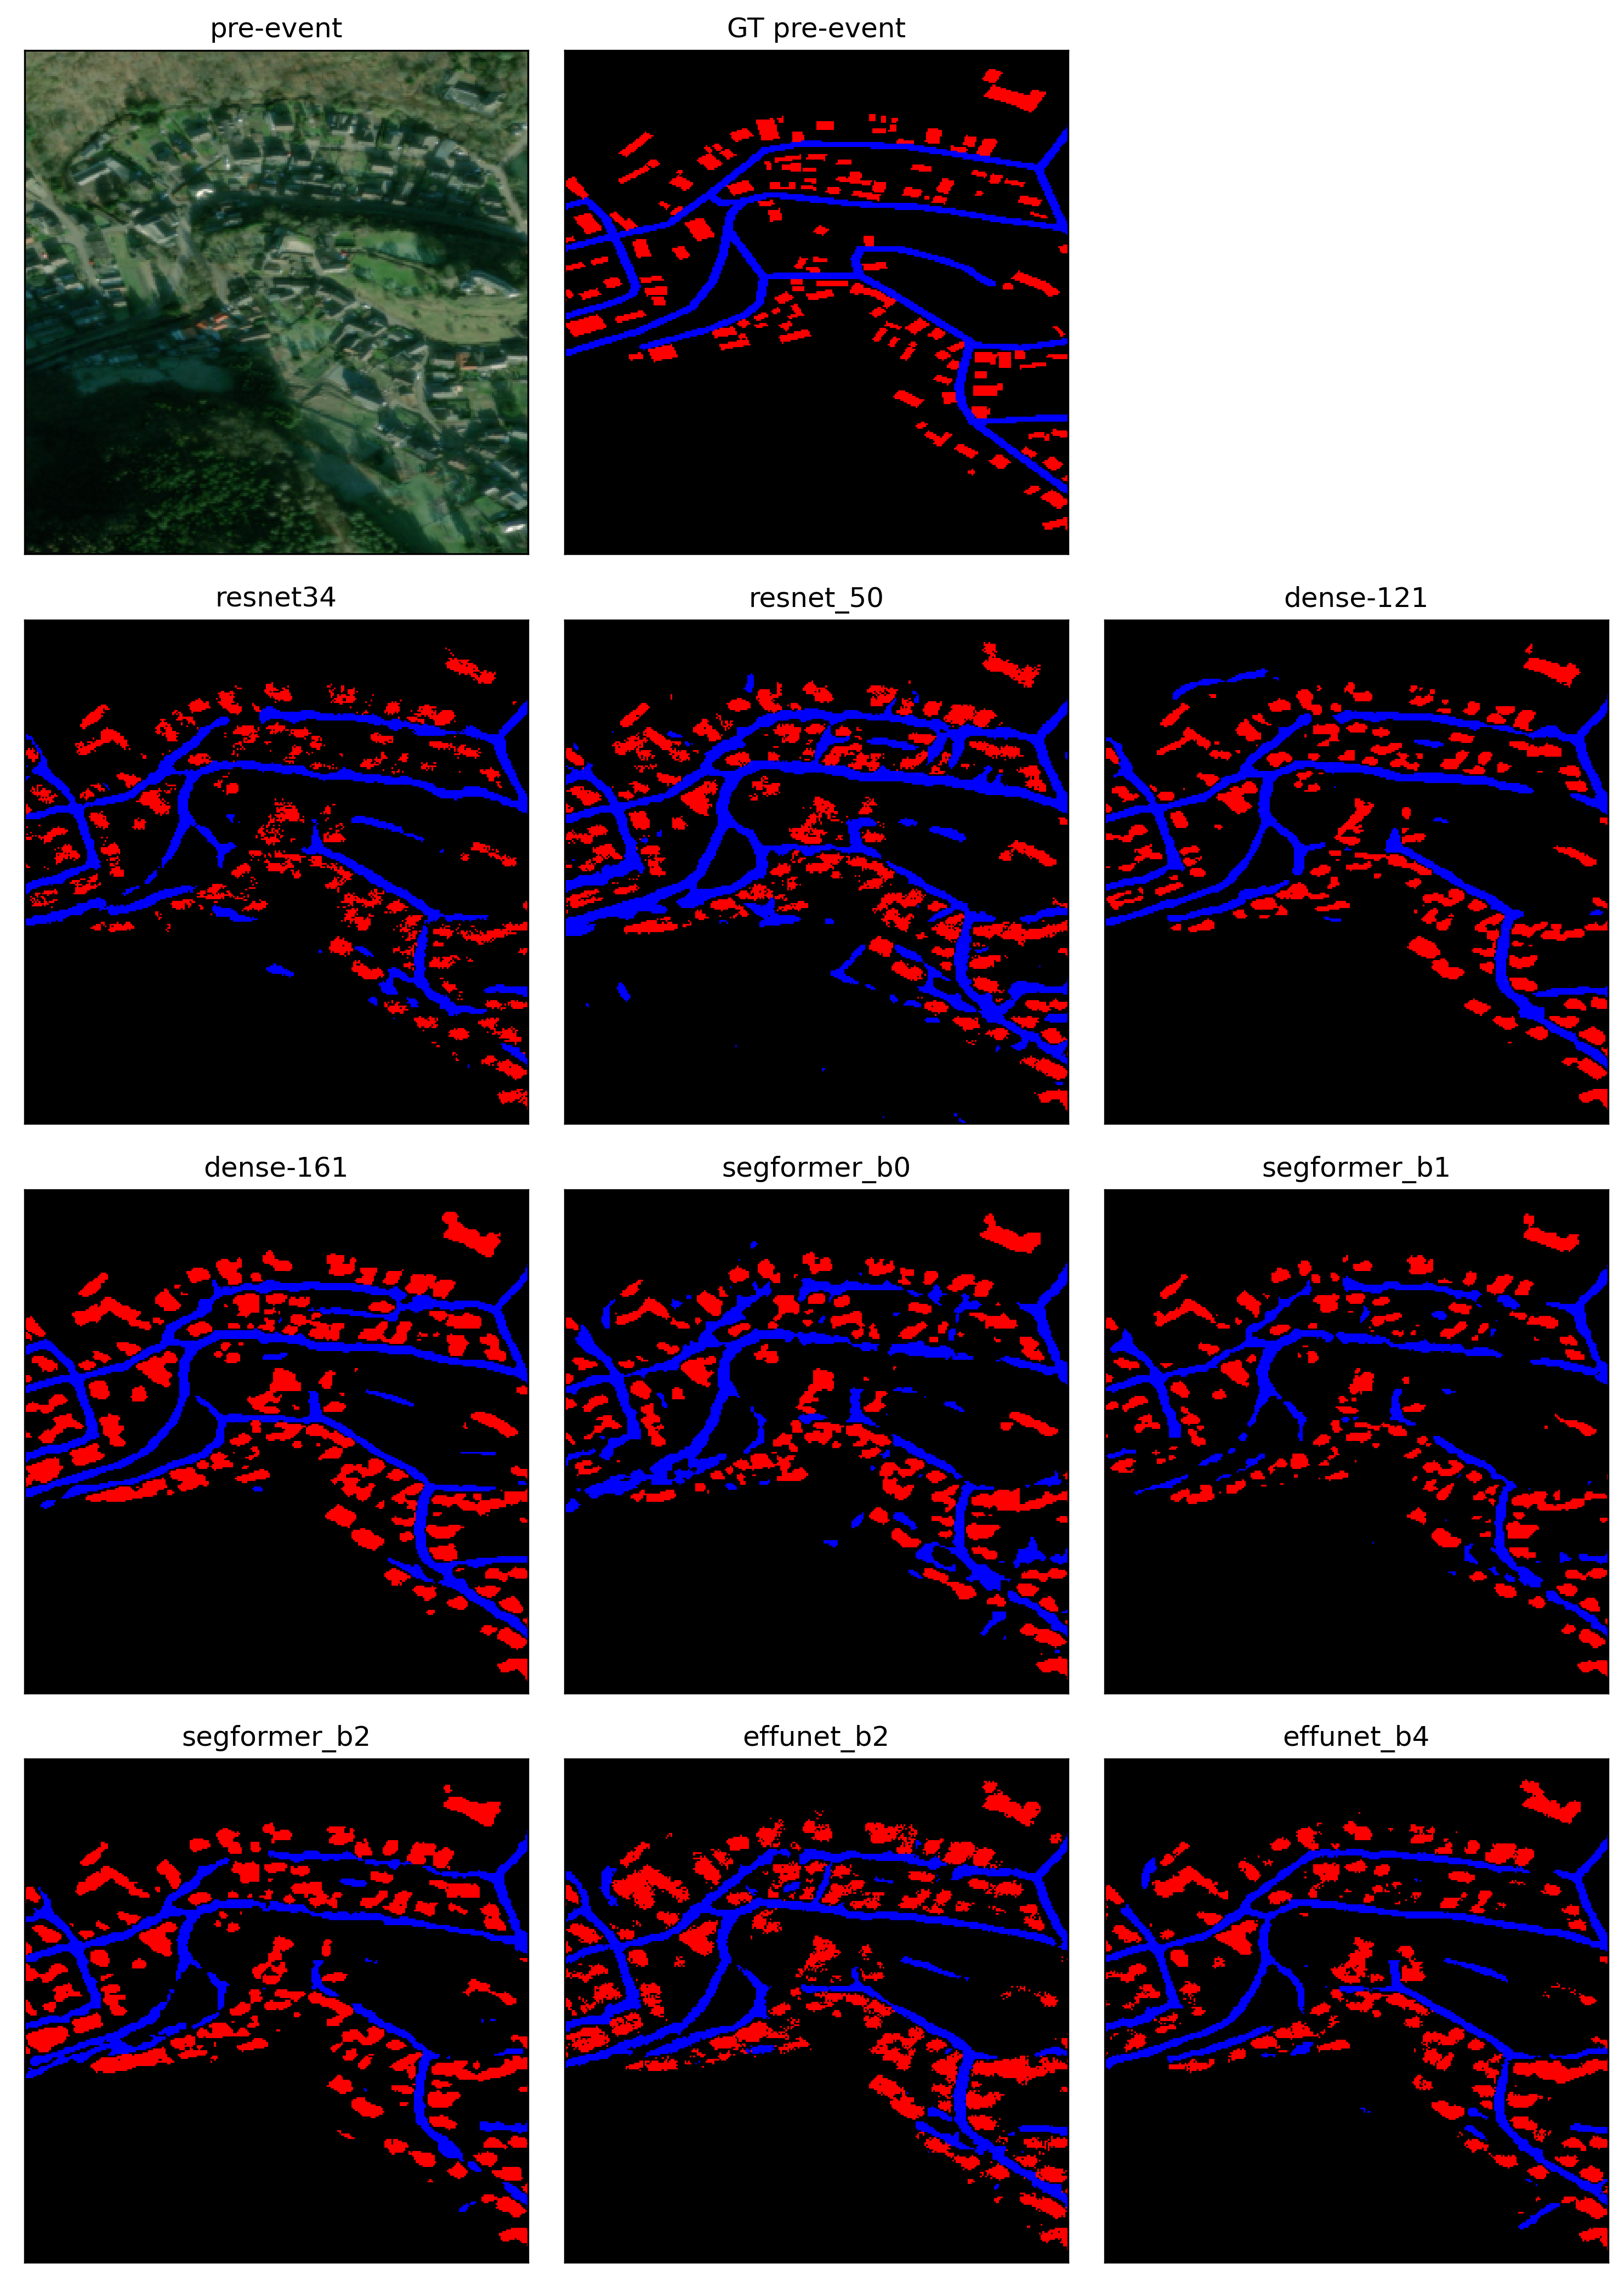
\includegraphics[width=2\linewidth]{final-report/figures/sample_images_foundation_1.png}
   \caption{Predictions across Foundation network models.}
   \label{fig:sample_images_foundation_1}
\end{figure}

\clearpage
\begin{figure}[t]
 \centering
  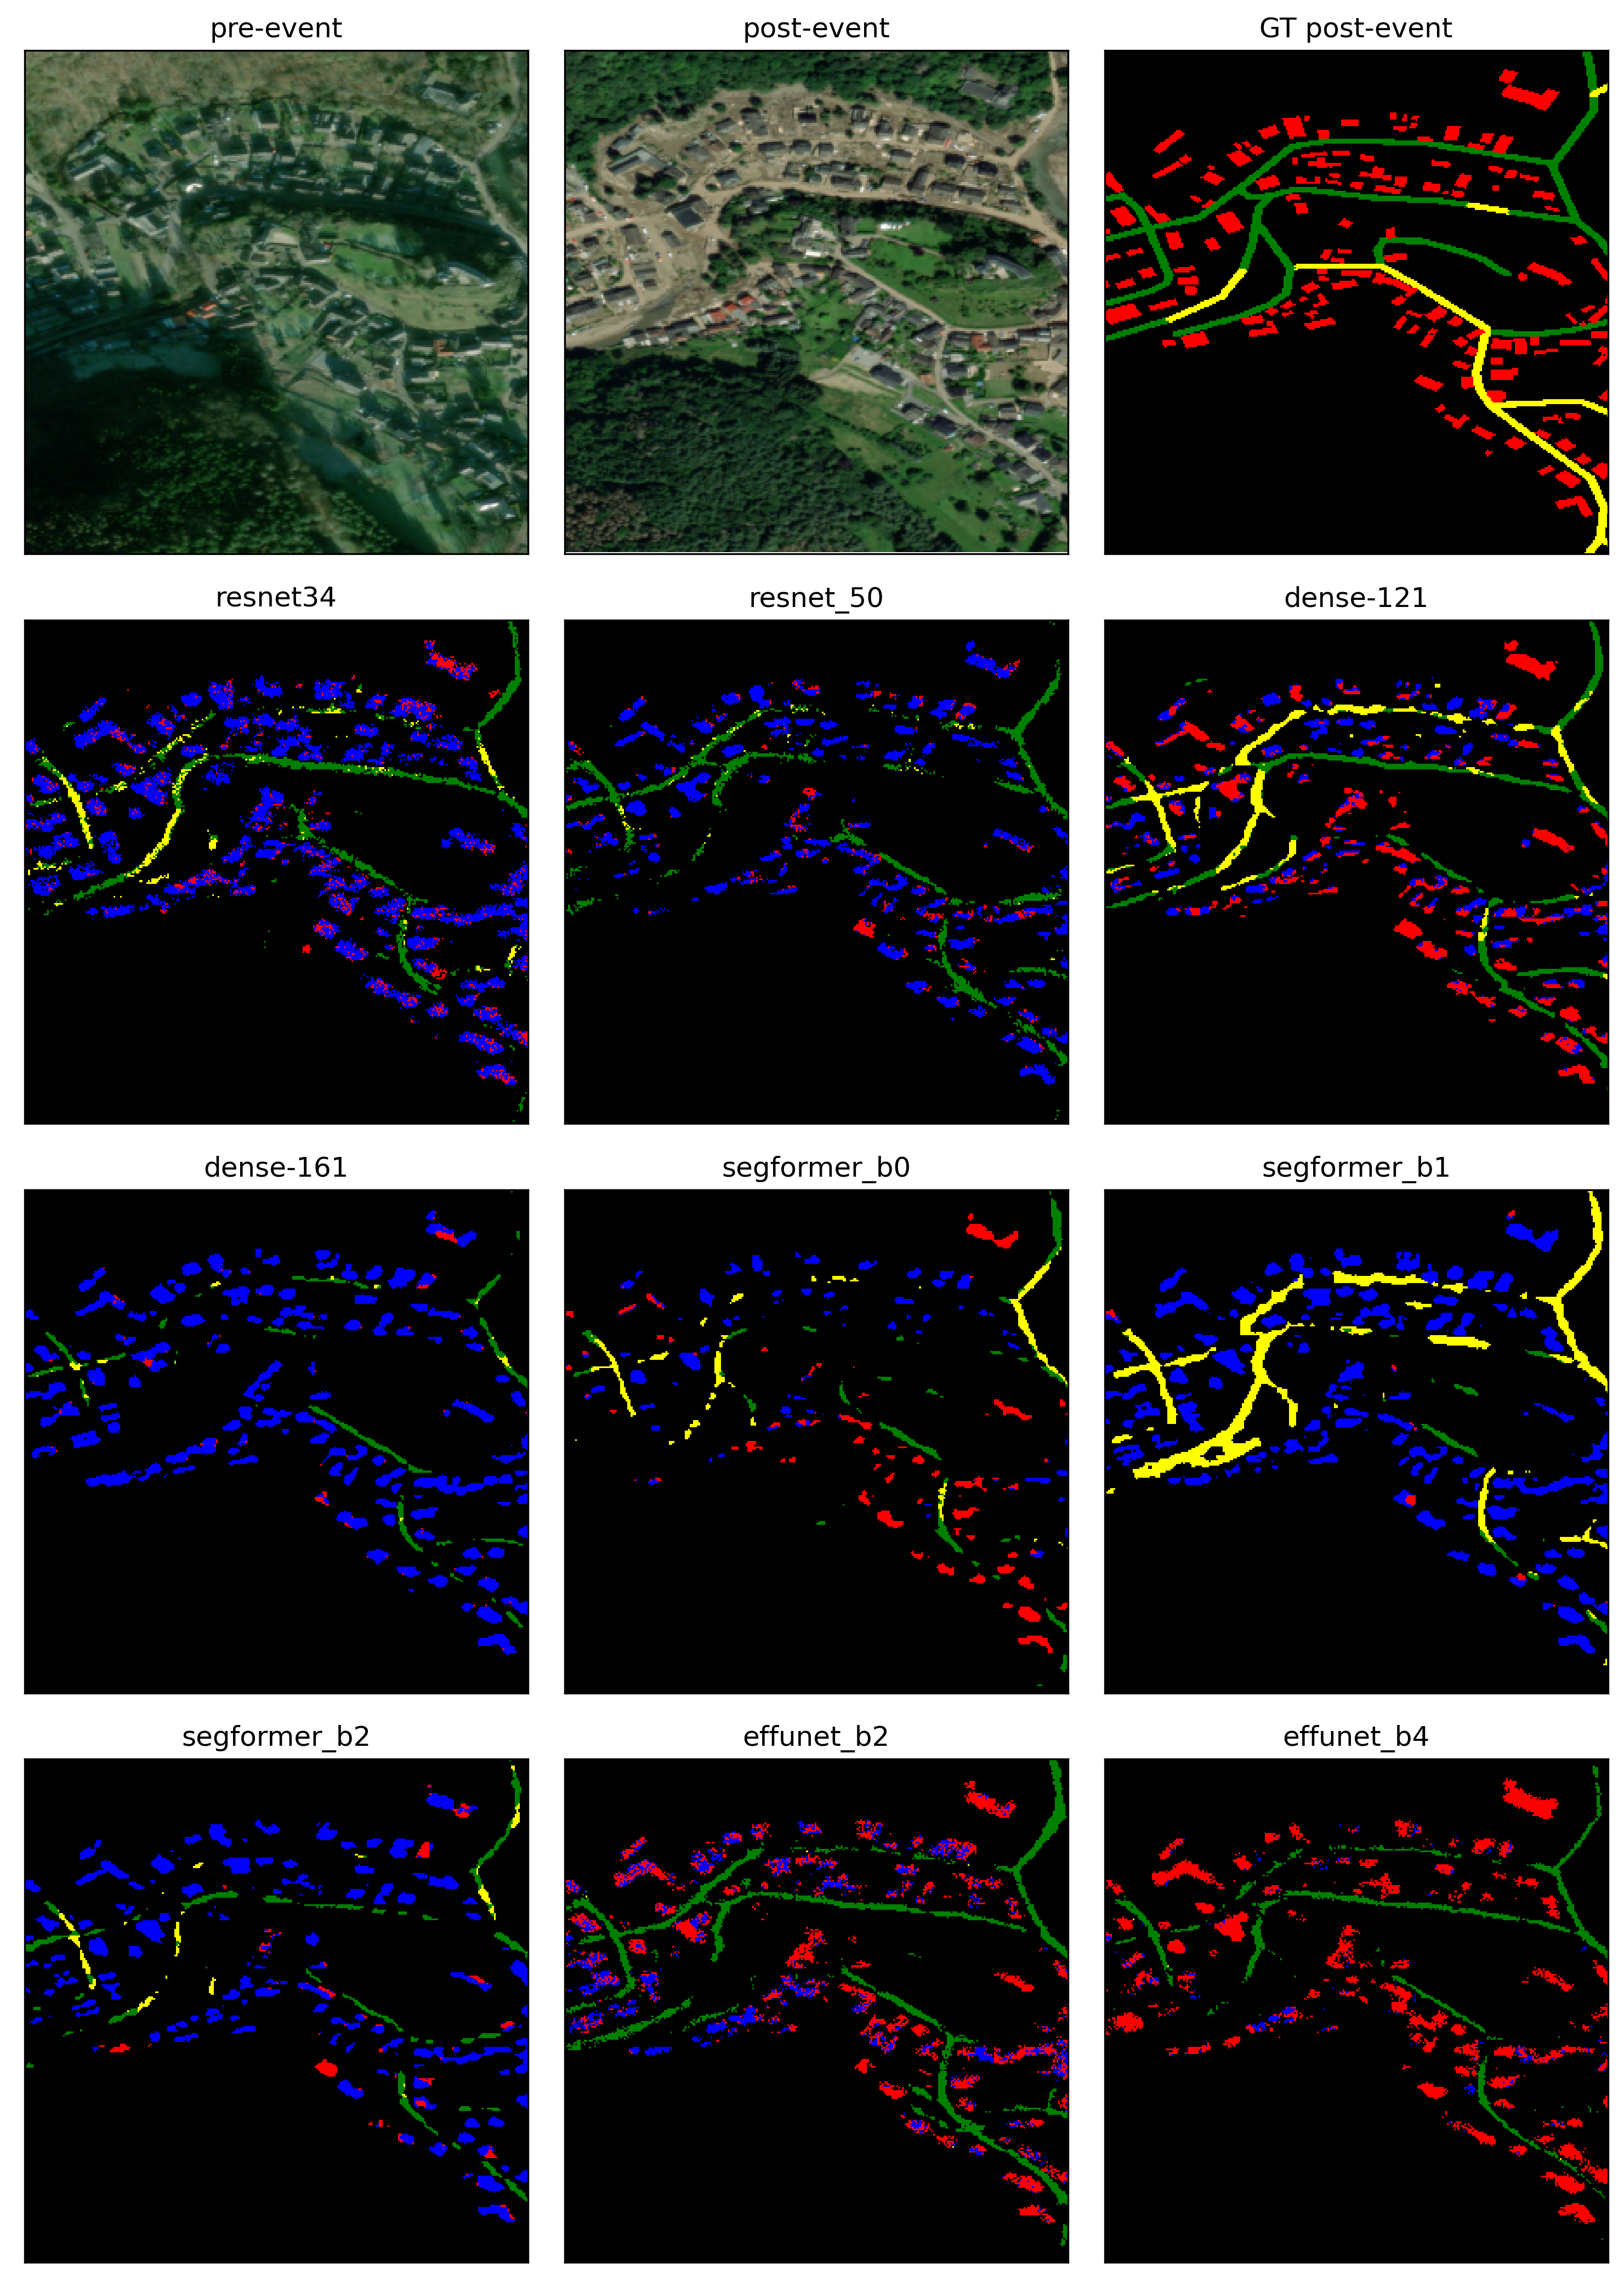
\includegraphics[width=2\linewidth]{final-report/figures/sample_images_flood_1.png}
  \caption{Predictions across Flood network models.}
  \label{fig:sample_images_flood_1}
\end{figure}


\clearpage
\begin{figure}[t]
  \centering
   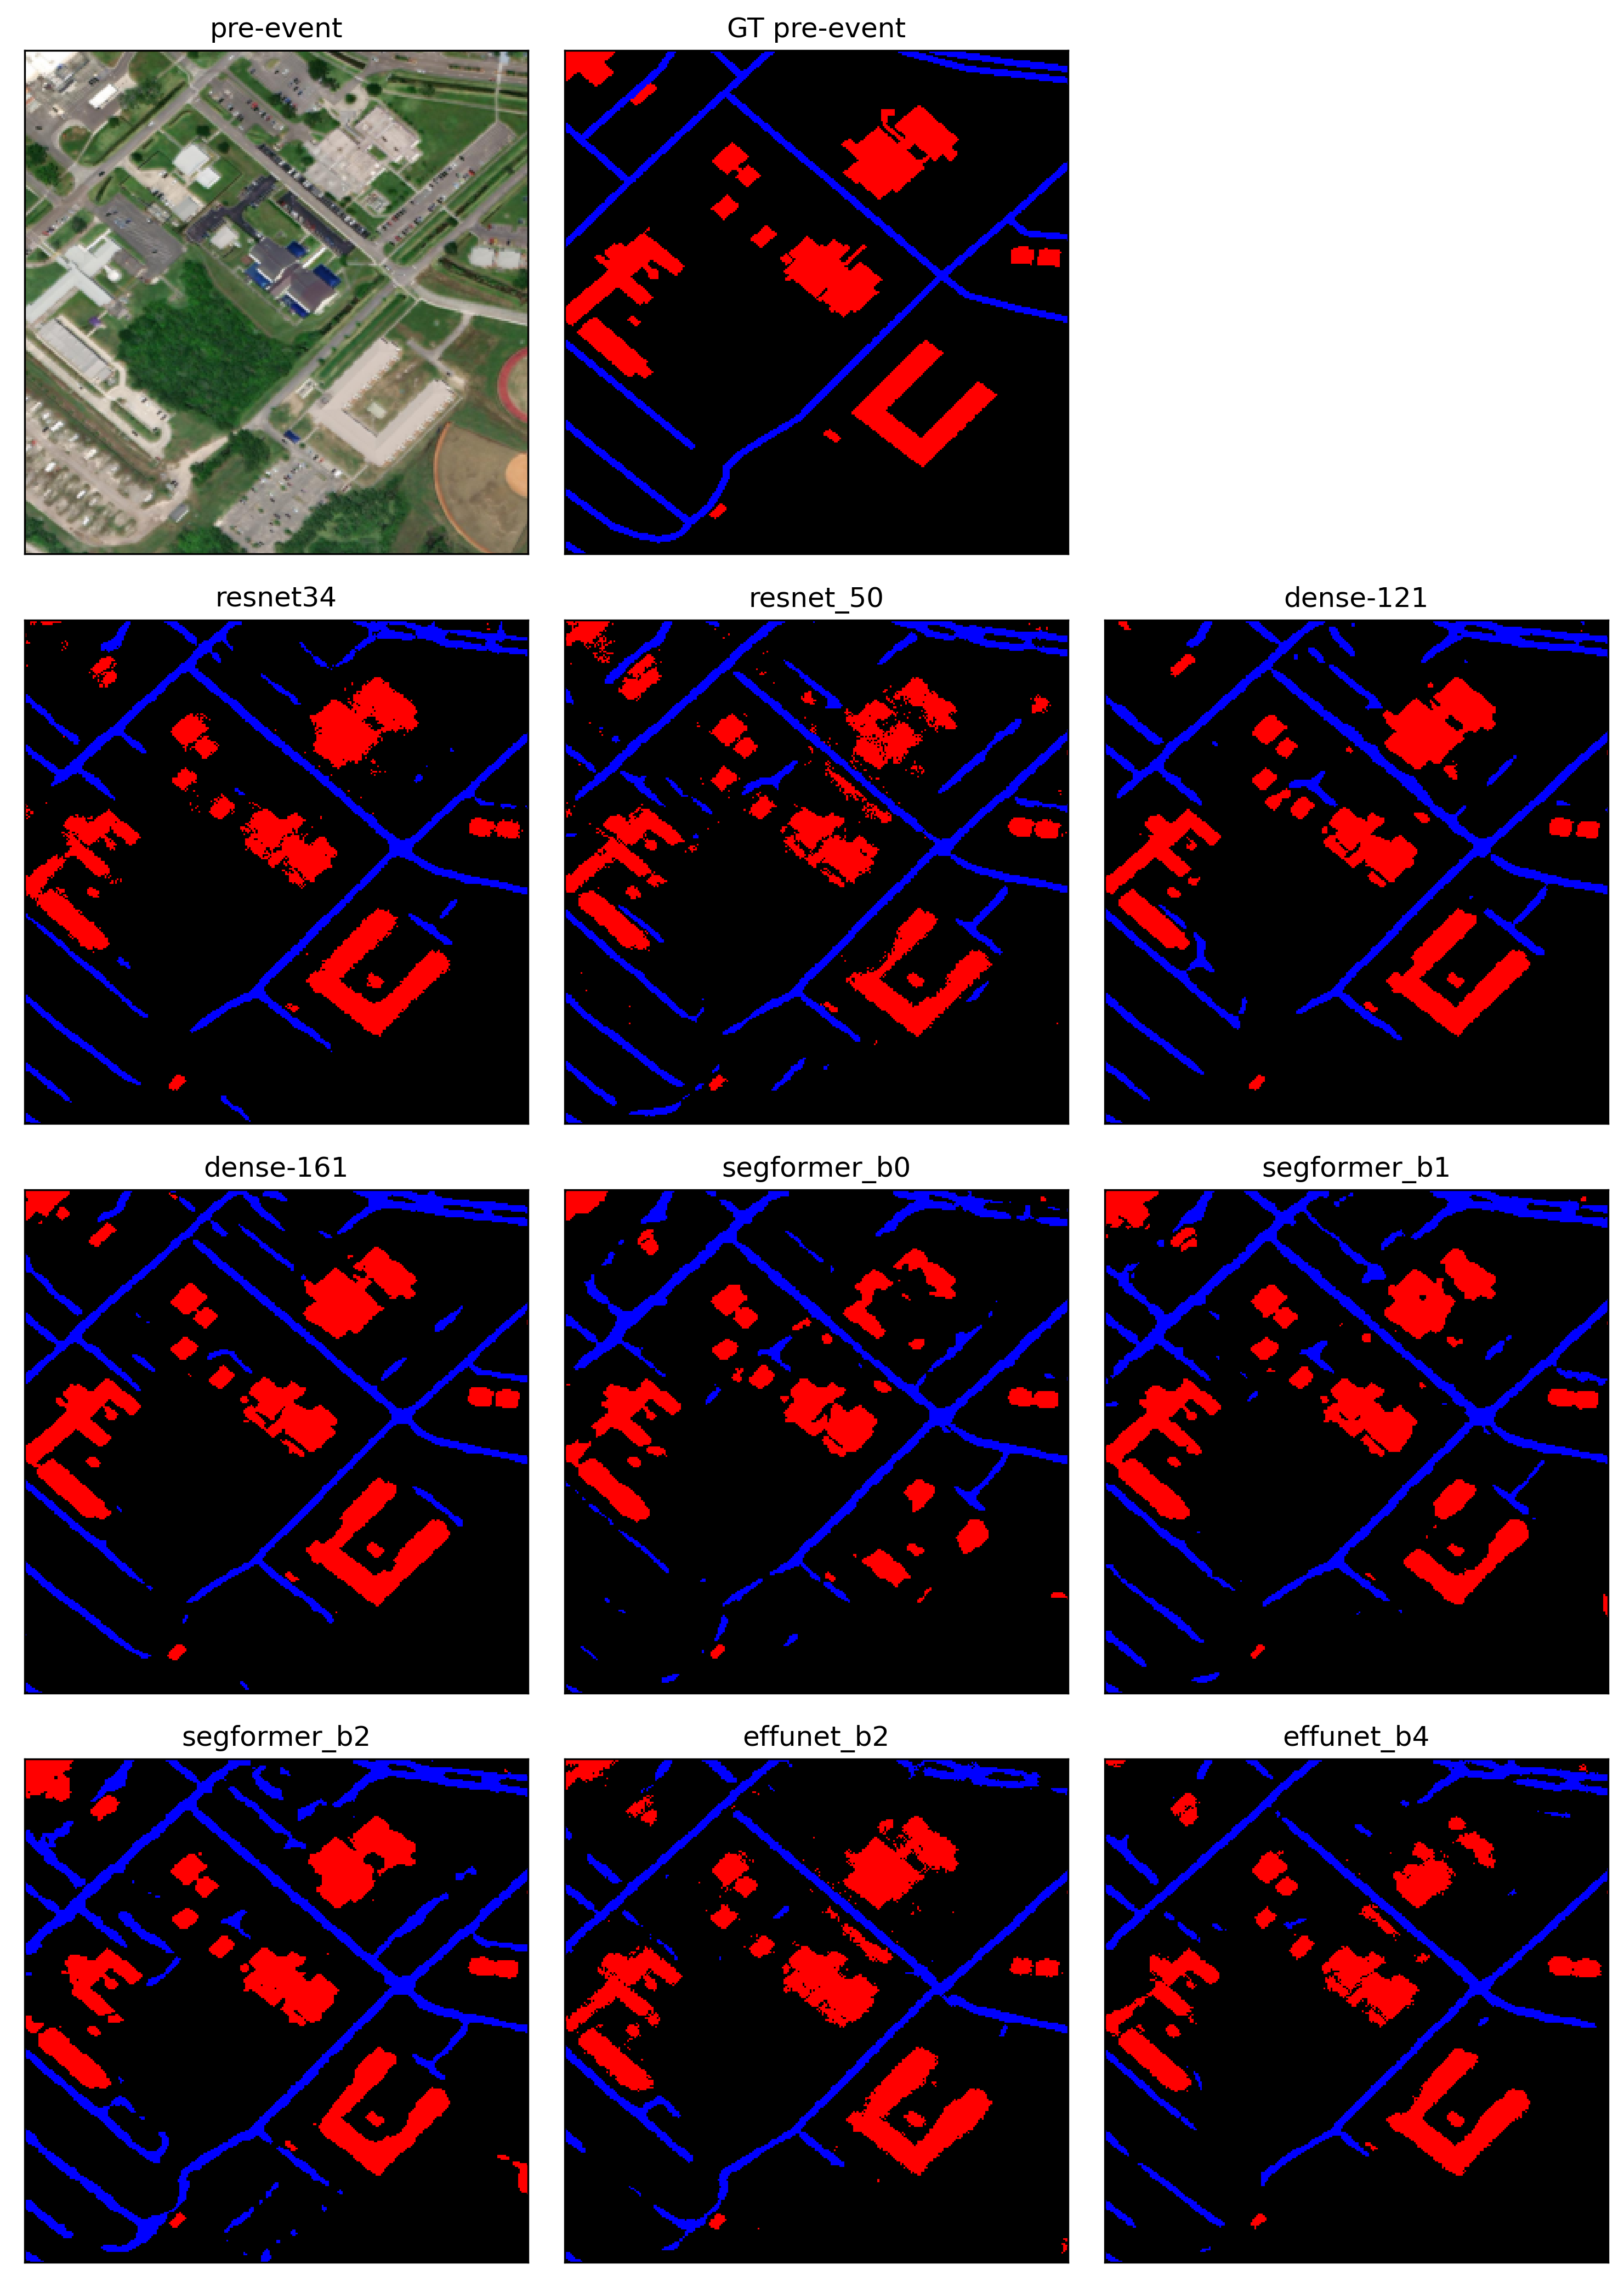
\includegraphics[width=2\linewidth]{final-report/figures/sample_images_foundation_2.png}
   \caption{Predictions across Foundation network models.}
   \label{fig:sample_images_foundation_2}
\end{figure}


\clearpage
\begin{figure}[t]
 \centering
  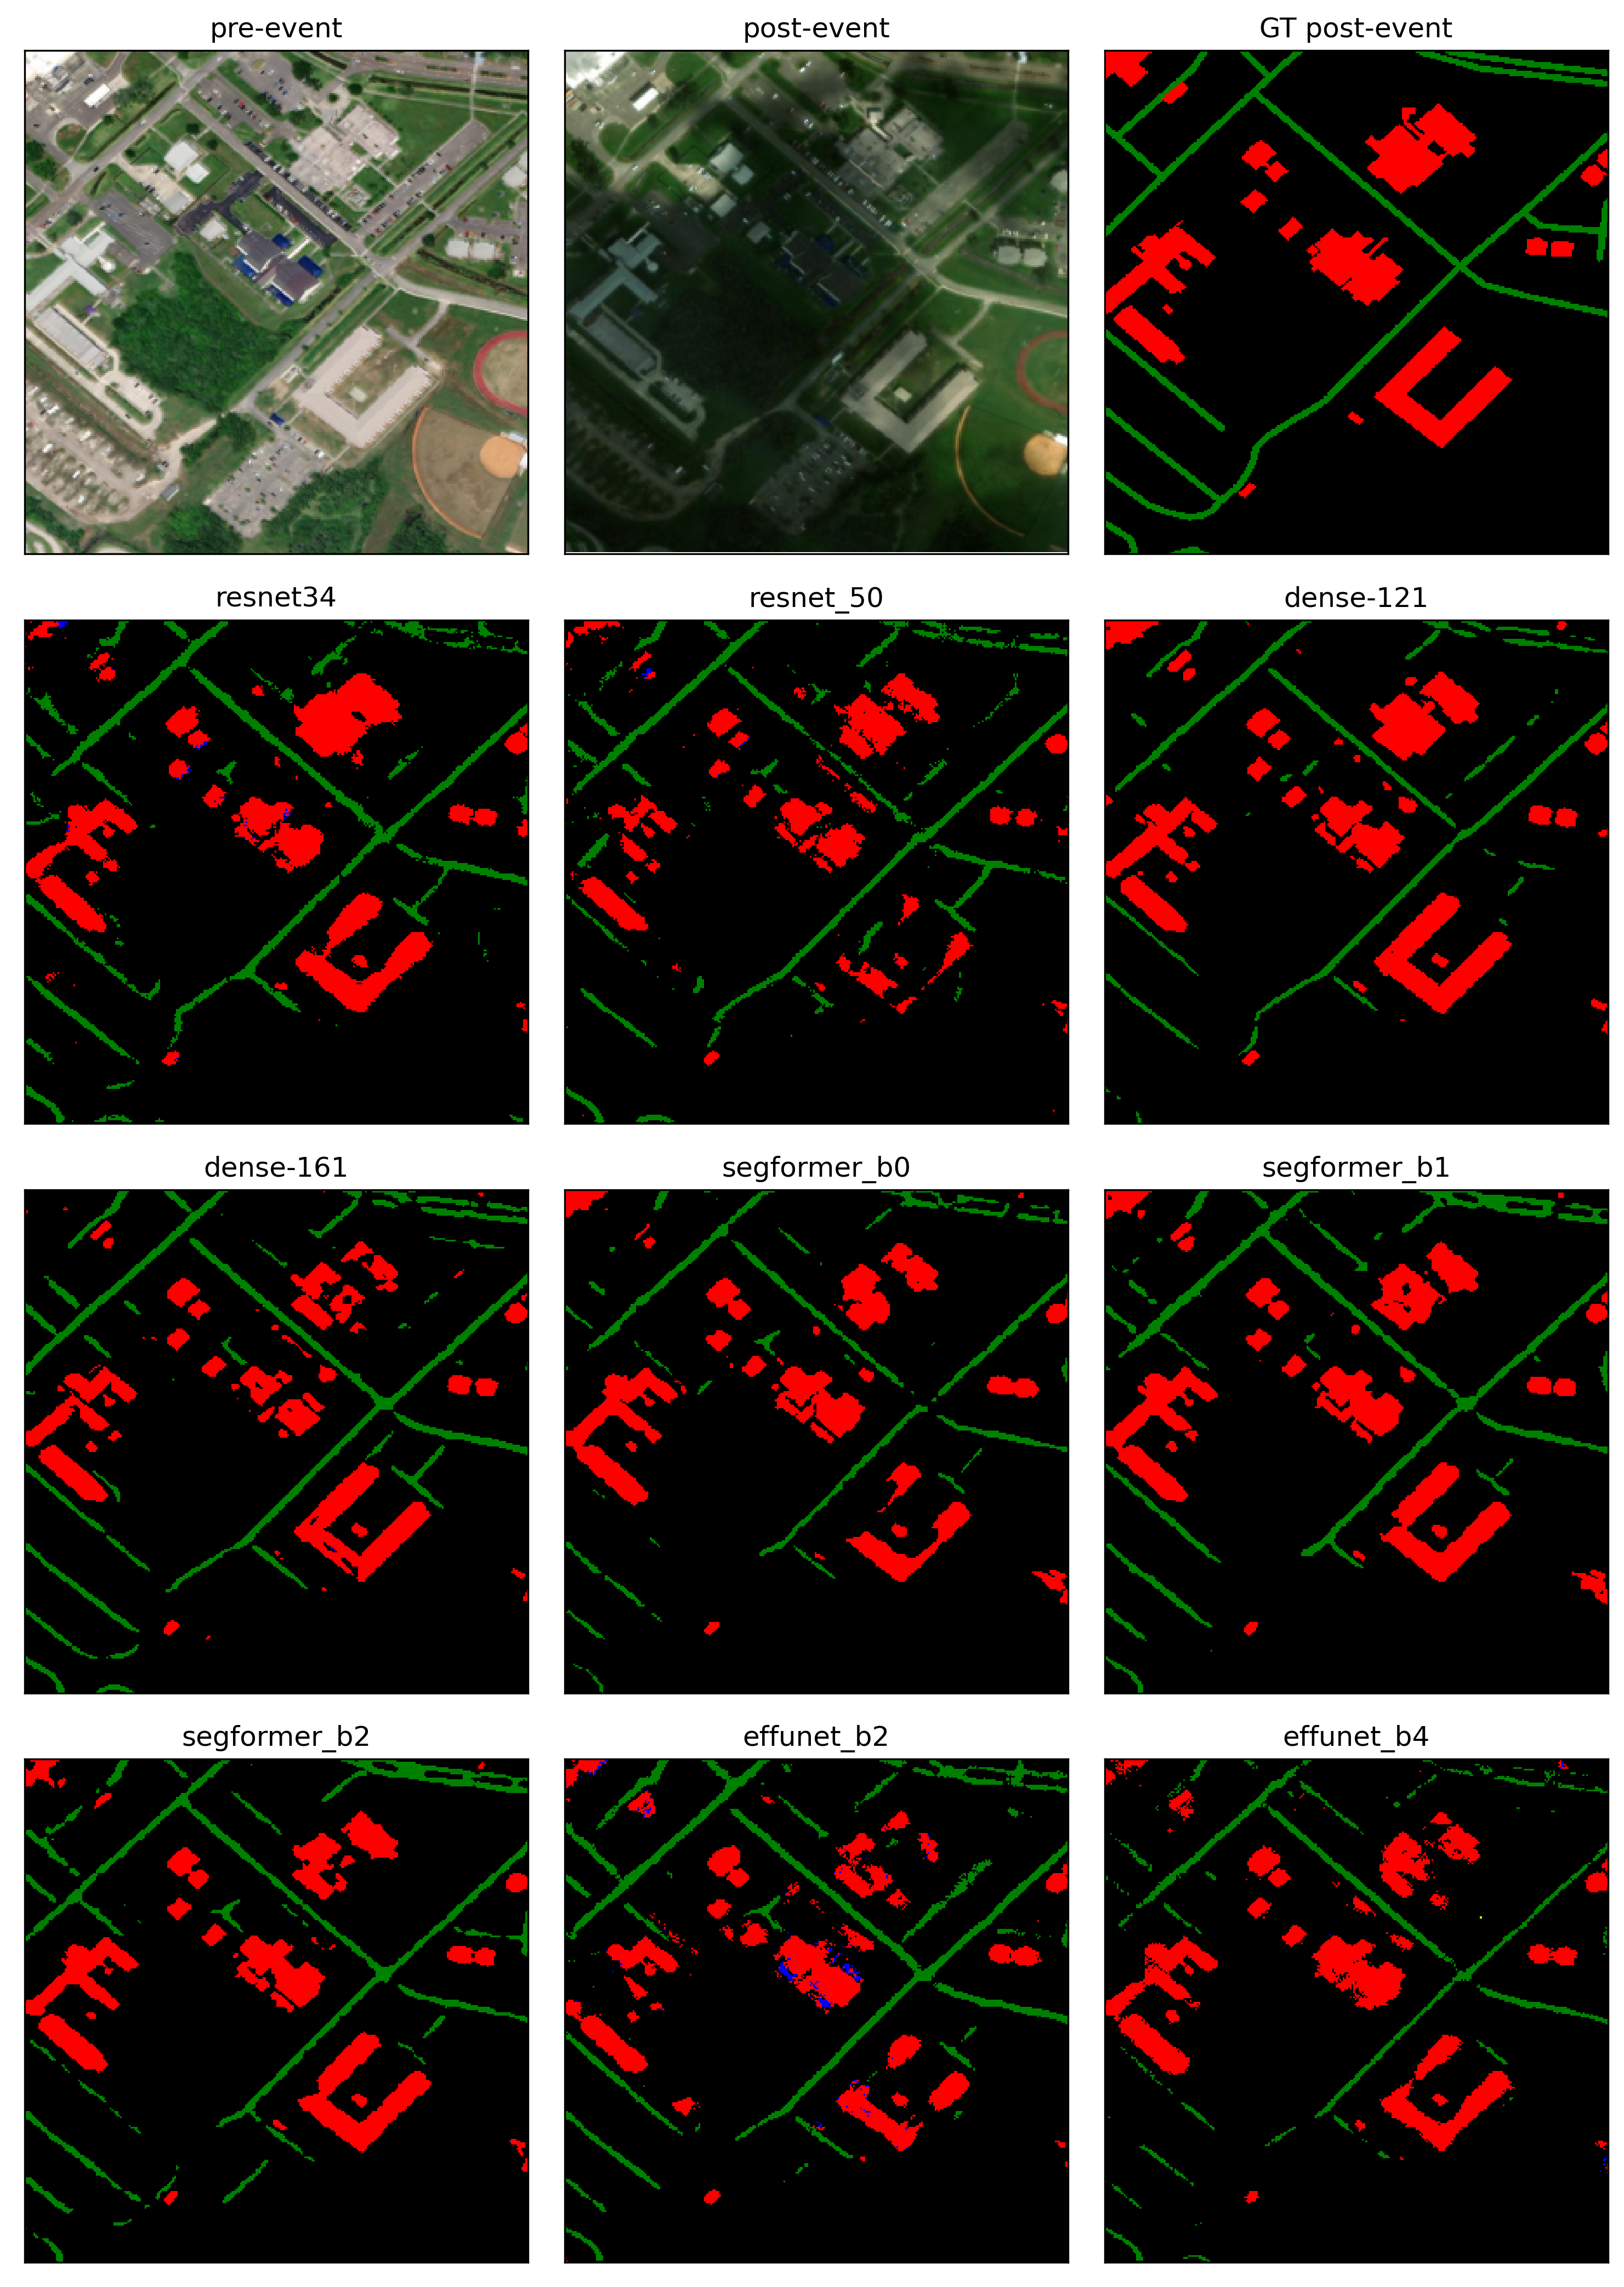
\includegraphics[width=2\linewidth]{final-report/figures/sample_images_flood_2.png}
  \caption{Predictions across Flood network models.}
  \label{fig:sample_images_flood_2}
\end{figure}


\end{document}
